\documentclass[diploma]{softlab-thesis}
\setlength\parindent{0pt}


\usepackage{listings}
\usepackage[section]{placeins}
%%%
%%%  The document
%%%

\begin{document}

%%%  Title page

\frontmatter

%%% TODO change
\title{Σχεδίαση και Επέκταση ενός Συστήματος Αυτόματης Αξιολόγησης Προγραμματιστικών Ασκήσεων}
\author{Αντώνιος Αγγελάκης}
\date{Μάρτιος 2018}
%%% TODO change
\datedefense{17}{3}{2018}

\supervisor{Νικόλαος Παπασπύρου}
\supervisorpos{Αν. Καθηγητής Ε.Μ.Π.}

\committeeone{Νικόλαος Παπασπύρου}
\committeeonepos{Αν. Καθηγητής Ε.Μ.Π.}
\committeetwo{Αριστείδης Παγουρτζής}
\committeetwopos{Αν. Καθηγητής Ε.Μ.Π.}
\committeethree{Γεώργιος Στάμου}
\committeethreepos{Αν. Καθηγητής Ε.Μ.Π.}

%%% TODO change
\TRnumber{CSD-SW-TR-42-18}  % number-year, ask nickie for the number
\department{Τομέας Τεχνολογίας Πληροφορικής και Υπολογιστών}

\maketitle


%%%  Abstract, in Greek

%%% TODO change
\begin{abstractgr}%

\begin{keywordsgr}
Συστήματα αξιολόγησης, Συστήματα διαχείρισης διαγωνισμών, CMS, Grader, PHP,
Python, Ανάπτυξη Λογισμικού, Λογισμικό ανοιχτού κώδικας, Ελεύθερο λογισμικό.
\end{keywordsgr}
\end{abstractgr}


%%%  Abstract, in English

%%% TODO change
\begin{abstracten}%

\begin{keywordsen}
Evaluation Systems, Contest management systems, CMS, Grader, PHP, Python,
Software development, Free and open source software.
\end{keywordsen}
\end{abstracten}


%%%  Acknowledgements

%%% TODO change
\begin{acknowledgementsgr}
\end{acknowledgementsgr}


%%%  Various tables

\tableofcontents
\listoftables
\listoffigures
\lstlistoflistings


%%%  Main part of the book

\mainmatter

\chapter{Εισαγωγή}

\section{Σκοπός}

Ο σκοπός της παρούσας διπλωματικής εργασίας είναι ο σχεδιασμός και η υλοποίηση
νέων δυνατοτήτων σε ένα σύστημα αυτόματης αξιολόγησης προγραμματιστικών
ασκήσεων. Το σύστημα που τροποποιήθηκε, όπως θα περιγραφεί παρακάτω,
χρησιμοποιείται τόσο από το Εργαστήριο Τεχνολογίας
Λογισμικού\footnote{http://grader.softlab.ntua.gr} όσο και από την Ελληνική
Εταιρεία Επιστημόνων και Επαγγελματιών Πληροφορικής και Επικοινωνιών
(ΕΠΥ)\footnote{http://hellenico.gr/grader} για τη διοργάνωση των Πανελλήνιων
Διαγωνισμών Πληροφορικής.

\bigskip

Το σύστημα αυτόματης αξιολόγησης (Grader) δέχεται τις υποβολές των
διαγωνιζομένων σε συγκεκριμένα προβλήματα που ανήκουν σε διαγωνισμούς,
ώστε να τις χαρακτηρίσει ενεργές ή όχι, αξιολογώντας
το αποτέλεσμα και την απόδοση τους σε συγκεκριμένα αρχεία ελέγχου.
Έπειτα, αφού κλείσουν οι υποβολές, επαναξιολογεί όλες τις ενεργές
υποβολές αυτόματα, ώστε να παράξει τα τελικά αποτελέσματα.

\bigskip

Ο Grader, στην πρότερη κατάσταση του, επέτρεπε μόνο τη δημιουργία
μεμονωμένων αρχείων ελέγχου και όχι συνδυαστικών ομάδων καθιστώντας
δύσκολη τη δημιουργία προβλημάτων με δυαδικά αποτελέσματα, π.χ. σωστό/λάθος.
Επιπροσθέτως, δεν υπήρχε η επιλογή για προσθήκη αρχείων ελέγχου αξιολόγησης
χωρίς επιρροή στην αρχική αξιολόγηση μιας υποβολής ως θετική ή αρνητική.

\bigskip

Η αρχική σχεδίαση του Grader είχε σκοπό τη δημιουργία ενός συστήματος αυτόματης
αξιολόγησης για διαγωνισμούς πληροφορικής, για να χρησιμοποιηθεί κυρίως από την
ΕΠΥ. Ως αποτέλεσμα, κάθε πρόβλημα αντιστοιχίζεται σε έναν μόνο διαγωνισμό και τόσο
οι διαγωνιζόμενοι όσο και οι υποβολές τους συνδέονται με το πρόβλημα. Για τη χρήση
του Grader σε εργασίες προγραμματισμού, θα μας ήταν προτιμότερο να υπάρχει
διαχωρισμός προβλήματος και υποβολών ώστε τα προβλήματα να μπορούν να
επαναχρησιμοποιηθούν ευκολότερα.

\bigskip

Επιπλέον, κρίθηκε σημαντικό να προστεθεί η Python στις διαθέσιμες γλώσσες
υποβολής καθώς πρόκειται για μια από τις πλέον δημοφιλείς γλώσσες και
χρησιμοποιείται ως εισαγωγική γλώσσα προγραμματισμού σε σημαντικά ακαδημαϊκά
ιδρύματα, όπως είναι το MIT και το Stanford \cite{website:popularpython}.
Τέλος, ήταν απαραίτητο να γίνουν μικρές βελτιστοποιήσεις στη λογική του Grader,
να προστεθούν μικρότερες δυνατότητες που επιδιώκουν τη βελτίωση της ευκολίας
χρήσης για διαγωνιζόμενους και διαχειριστές και να αντικατασταθούν
απαρχαιωμένα, χωρίς ενεργή ανάπτυξη εργαλεία/βιβλιοθήκες για την επίτευξη
καλύτερης απόδοσης και ασφάλειας.

\newpage

\section{Δομή Εργασίας}

Η εργασία ακολουθεί την παρακάτω δομή:

\begin{itemize}
  \item \textbf{Κεφάλαιο 2}: Συστήματα Αυτόματης Αξιολόγησης \\
    Παρουσιάζουμε κάποια γνωστά συστήματα αυτόματης αξιολόγησης με παρόμοια
    λειτουργία και σκοπό όπως ο Grader. Γίνεται επίσης μια σύγκριση με τις
    δυνατότητες του παρόντος συστήματος.
  \item \textbf{Κεφάλαιο 3}: Περιγραφή Grader - Kewii \\
    Περιγράφεται η υπάρχουσα δομή και λειτουργία του Grader, αναλύοντας τα
    διαφορετικά μέρη του και τις σχέσεις μεταξύ τους.
  \item \textbf{Κεφάλαιο 4}: Προσθήκη Ομάδων Αρχείων Ελέγχου \\
    Αναλύεται η σχεδιαστική λογική και η υλοποίηση της νέας δυνατότητας του
    συστήματος, για ομαδοποίηση των αρχείων ελέγχου των προβλημάτων.
  \item \textbf{Κεφάλαιο 5}: Σχεδίαση για διαχωρισμό Προβλημάτων - Διαγωνισμών \\
    Περιγράφεται η υλοποίηση της συγκεκριμένης τροποποίησης για την βελτίωση της
    λειτουργίας του Grader στο πλαίσιο προγραμματιστικών ασκήσεων.
  \item \textbf{Κεφάλαιο 6}: Λοιπές Προσθήκες \\
    Στο συγκεκριμένο κεφάλαιο παρατίθενται βελτιώσεις και προσθήκες μικρότερου
    μεγέθους.
  \item \textbf{Κεφάλαιο 7}: Συμπεράσματα \\
    Στο τελευταίο κεφάλαιο παρουσιάζονται κάποιες παρατηρήσεις σχετικά με τη
    διπλωματική και αναφέρονται ιδέες για περαιτέρω ανάπτυξη του συστήματος.
\end{itemize}


\chapter{Συστήματα Αυτόματης Αξιολόγησης}

O Grader έχει σκοπό τη διοργάνωση προγραμματιστικών διαγωνισμών ή εργασιών
με αυτόματο τρόπο υποβολής, εκτέλεσης και αξιολόγησης των λύσεων. Το παρόν
σύστημα είναι κλειστού κώδικα, όμως θα είχε σημασία να μελετήσουμε συστήματα
με παρόμοια λειτουργία ώστε να δούμε ομοιότητες και διαφορές με το δικό μας.

\bigskip

Προτιμήθηκε να ελεγχθούν μόνο συστήματα ελεύθερου λογισμικού και ανοιχτού
κώδικα διότι μας προσφέρουν σημαντικά πλεονεκτήματα. Αρχικά, μας επιτρέπουν να
ερευνήσουμε τον τρόπο που είναι σχεδιασμένα και να πάρουμε ιδέες για τον
Grader. Επιπλέον, είναι πιθανό να παρέχουν καλύτερη ασφάλεια, καθώς
οποιοσδήποτε μπορεί να ελέγξει τον κώδικα για ευπάθειες. Φυσικά, το τελευταίο
ισχύει υπό την προϋπόθεση ότι υπάρχει πρωτοβουλία για έλεγχο της ασφάλειας
(audit), αφού η απλή δημοσιοποίηση του κώδικα μπορεί να δίνει την ψευδαίσθηση
(όπως αναφέρεται στο \cite{hansen2002open}). Τέλος, η σύγκριση του Grader με τα
συγκεκριμένα συστήματα έχει μεγάλη σημασία γιατί θα μπορούσε οποιοδήποτε από
αυτά να τον αντικαταστήσει χωρίς μεγάλο κόστος (κυρίως αυτό της μετάβασης) σε
περίπτωση που θεωρηθεί ανώτερο.

\bigskip

Τα συστήματα που θα μελετηθούν είναι τα παρακάτω:

\begin{itemize}
    \setlength\itemsep{0em}
    \item CMS
    \item Mooshak 2.0
    \item CATS
\end{itemize}

Και τα 3 έχουν σχεδιαστεί με σκοπό τη διεξαγωγή προγραμματιστικών διαγωνισμών,
ολυμπιάδων πληροφορικής, αλλά και χρήση για εργαστηριακές ασκήσεις και
εργασίες.

\section{CMS}

Το πρώτο σύστημα που θα μελετήσουμε είναι το Contest Management System, CMS εν
συντομία. Πρόκειται για ένα κατανεμημένο σύστημα διαχείρισης και διεξαγωγής
διαγωνισμών το οποίο σχεδιάστηκε αρχικά για την Διεθνή Ολυμπιάδα Πληροφορικής
του 2012. Αποτελείται από ένα πλήθος μικρο-υπηρεσιών που συνθέτουν το συνολικό
σύστημα.

\bigskip

Είναι, πιθανότατα, το πιο ολοκληρωμένο σύστημα για διαγωνισμούς δεδομένου του
μεγάλου αριθμού διαπιστευτηρίων που κατέχει, συμπεριλαμβανομένης της χρήσης του
σε όλες σχεδόν τις Διεθνείς Ολυμπιάδες από το 2012. Οι δημιουργοί του είχαν ως
στόχο τη δημιουργία ενός συστήματος ασφαλούς, ανθεκτικού σε σφάλματα λογισμικού
και υλικού, ανοιχτού, επεκτάσιμου και εύχρηστου.

\bigskip

Η ανάπτυξη του ξεκίνησε το 2010 και πλέον βασίζεται στην κοινότητα για
συνεισφορά στην ανάπτυξη του, στην προσθήκη μεταφράσεων και στη βελτίωση του
documentation. H άδεια που χρησιμοποιεί είναι η AGPL-3+ (GNU Affero General
Public License), η οποία επιτρέπει εμπορική χρήση, τροποποίηση και διανομή, με
την προϋπόθεση να παραμείνει η ίδια άδεια και να δημοσιευτεί ο πηγαίος κώδικας.

\subsection{Τεχνικά Χαρακτηριστικά}

Το CMS είναι γραμμένο σε Python και αποτελείται από πολλά μικρά κομμάτια που
αναλαμβάνουν μια ξεχωριστή λειτουργία. Αυτά μπορούν να έχουν εγκατασταθεί σε
διαφορετικούς εξυπηρετητές, σε απομακρυσμένα συστήματα. Οι υπηρεσίες-κομμάτια, από
τα οποία αποτελείται είναι τα παρακάτω:

\begin{itemize}
    \setlength\itemsep{0em}
    \item LogService \\
      Συλλέγει σε ένα μέρος όλα τα μηνύματα καταγραφής.
    \item ResourceService \\
      Λαμβάνει δεδομένα για όλες τις υπηρεσίες που τρέχουν και μπορεί να τις
      ξεκινήσει ταυτόχρονα.
    \item Checker \\
      Ελέγχει την κατάσταση των υπηρεσιών.
    \item EvaluationService \\
      Οργανώνει την ουρά υποβολών και διανέμει τις εργασίες στους Workers.
    \item Worker
      Εκτελεί τις εργασίες σε ένα αποκλεισμένο περιβάλλον.
    \item ScoringService \\
      Συλλέγει τα αποτελέσματα των εκτελέσεων και τα αξιολογεί για να παράξει
      τις βαθμολογίες.
    \item ProxyService \\
      Στέλνει τις βαθμολογίες στον εξυπηρετητή Αποτελεσμάτων.
    \item PrintingService \\
      Αναλαμβάνει την εκτύπωση των εγγράφων.
    \item ContestWebServer \\
      Ο εξυπηρετητής της ιστοσελίδας του διαγωνισμού, με τον οποίο αλληλεπιδρούν
      οι διαγωνιζόμενοι.
    \item AdminWebServer \\
      Ο εξυπηρετητής της ιστοσελίδας διαχείρισης του διαγωνισμού.
    \item RankingWebServer \\
      Ο εξυπηρετητής της ιστοσελίδας εμφάνισης των αποτελεσμάτων.
\end{itemize}

\bigskip

Όλες οι παραπάνω λειτουργίες αλληλεπιδρούν μεταξύ τους με τον τρόπο που φαίνεται
στην εικόνα 2.1.

\begin{figure}
  \centering
  \includegraphics[scale=0.4,trim=4 4 4 4,clip]{Figures/cmsarchitecture.png}
  \caption[Η αρχιτεκτονική του CMS]{Οι υπηρεσίες του CMS και οι σχέσεις μεταξύ τους.
  Βασισμένο στο σχήμα 1 του \cite{maggiolo2012introducing}.}
\end{figure}

\bigskip

Ο κύκλος διεξαγωγής ενός διαγωνισμού είναι γνώριμος. Αφού στηθούν όλες οι
απαραίτητες υπηρεσίες, οι διαχειριστές μπορούν να δημιουργήσουν το διαγωνισμό
μέσω του AdminWebServer, μαζί με τα προβλήματα και τα τεστ που περιέχει.
Έπειτα, κάθε διαγωνιζόμενος αλληλεπιδρά με τη σελίδα υποβάλλοντας τις λύσεις
του. Αυτές αποθηκεύονται στο δίσκο μέχρι να δοθούν σε κάποιο Worker από το
EvaluationService και να εκτελεστούν στο ασφαλές περιβάλλον. Σε εκείνο το
σημείο αναλαμβάνει τα ηνία το ScoringService που αξιολογεί τις εκτελέσεις και
στέλνει τα αποτελέσματα στο RankingWebServer, ώστε να ανανεωθεί με την
τελευταία εικόνα.

\bigskip

Η βάση που χρησιμοποιεί το CMS είναι PostgreSQL και η λειτουργία του βασίζεται
στα χαρακτηριστικά της, οπότε μόνο αυτή υποστηρίζεται. Οι γλώσσες προγραμματισμού
που υποστηρίζει η ευσταθής έκδοση του είναι οι: C, C++, PHP, Pascal, Java και
Python2. Στην τελευταία έκδοση υπό ανάπτυξη (development) υποστηρίζονται επίσης
C\#, Haskell, Python3 και Rust. Για την επέκταση του με παραπάνω γλώσσες αρκεί
η προσθήκη ενός αρχείου προδιαγραφών για κάθε νέα γλώσσα.


\subsection{Εγκατάσταση και Χρήση}

Η εγκατάσταση προϋποθέτει την ύπαρξη πλήθους εργαλείων για την υποστήριξη των
γλωσσών και του συστήματος. Όπως έχει αναφερθεί, το CMS αποτελείται από πολλές
διαφορετικές υπηρεσίες, οι οποίες πρέπει να τρέχουν σε ένα ή παραπάνω μηχανήματα
για την πλήρη λειτουργία. Χάρη στην ύπαρξη του ResourceService όλες οι υπηρεσίες
ενός μηχανήματος μπορούν να εκκινήσουν ταυτόχρονα ώστε να μειωθεί η χρονοβόρα
εργασία.

\bigskip

Για να τρέξει επίσης το σύστημα θα πρέπει να γίνουν οι απαραίτητες ρυθμίσεις
στην βάση αλλά και στο CMS. Μόλις ολοκληρωθεί κι αυτό το βήμα, οι διαχειριστές
μπορούν να δημιουργήσουν διαγωνισμούς και προβλήματα με τρεις τρόπους: μέσω της
διεπαφής Admin, κατευθείαν από το σύστημα αρχείων τους περιγράφοντας με αρχείο
προδιαγραφών τη μορφή τους ή με απευθείας εισαγωγή προηγούμενου διαγωνισμού που
εξάχθηκε.

\bigskip

Οι διαγωνιζόμενοι συμμετέχουν στο διαγωνισμό μέσω της σελίδας του
ContestWebServer. Εκεί βλέπουν για κάθε πρόβλημα την περιγραφή του και όλα
τα σχετικά με αυτό στοιχεία και μπορούν να υποβάλλουν τις λύσεις τους. Ένα
ενδιαφέρον χαρακτηριστικό είναι ότι οι διαγωνιζόμενοι μπορούν να δημιουργούν
δικά τους αρχεία ελέγχου, στα οποία θα ελεγχθεί η λύση τους. Επιπλέον, υπάρχει
η δυνατότητα χρήσης tokens, τα οποία μοιράζονται στους διαγωνιζόμενους και
περιορίζουν τις φορές που μπορούν να δουν τα αναλυτικά αποτελέσματα της
υποβολής τους σε φανερά και κρυφά αρχεία ελέγχου.

\bigskip

Ακολουθούν φωτογραφίες από τις διεπαφές του διαγωνισμού, του Admin και της σελίδας
των αποτελεσμάτων.

\bigskip

\begin{figure}
  \centering
  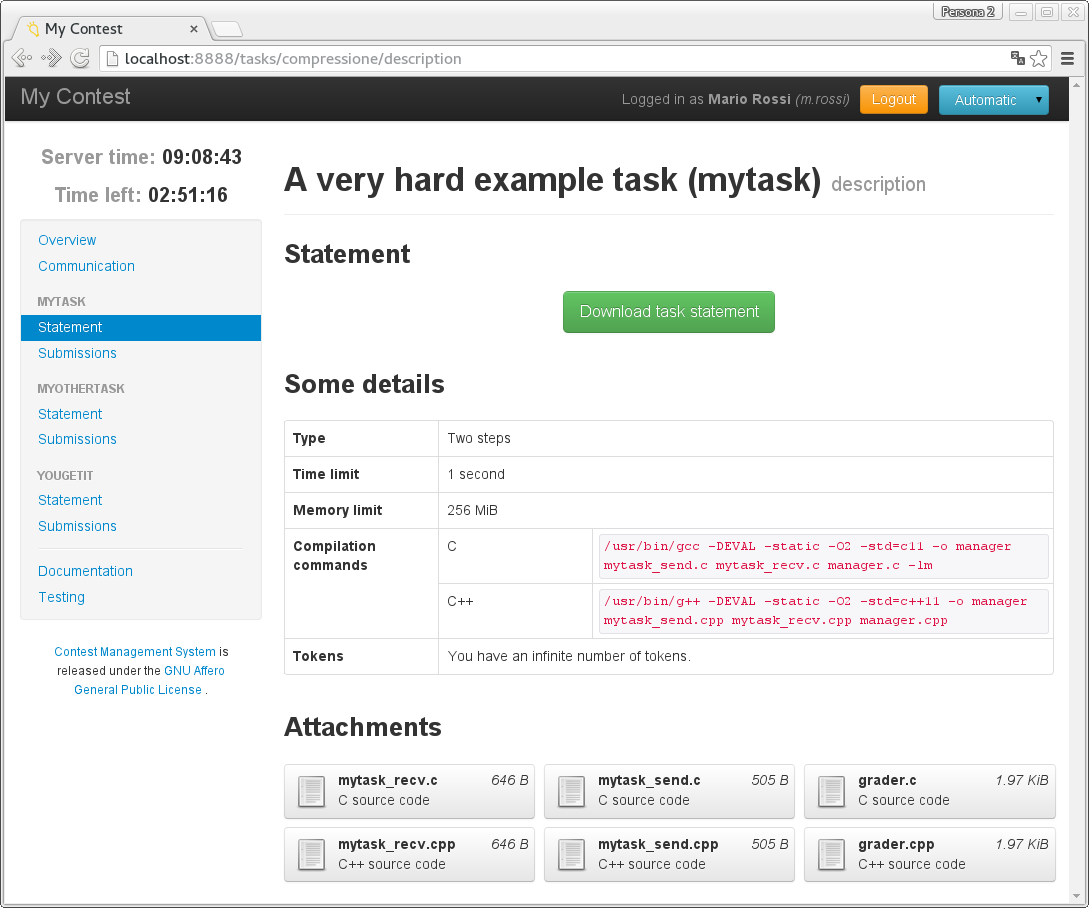
\includegraphics[scale=0.3,trim=4 4 4 4,clip]{Figures/cmscontestant.png}
  \caption[Οθόνη προβλήματος CMS]{Η οθόνη ενός προβλήματος, όπως τη βλέπει ένας
  διαγωνιζόμενος. Διακρίνονται τα στοιχεία του προβλήματος και όλα τα
  επισυναπτόμενα. Πηγή: https://cms-dev.github.io/screenshots.html}
\end{figure}

\begin{figure}
  \centering
  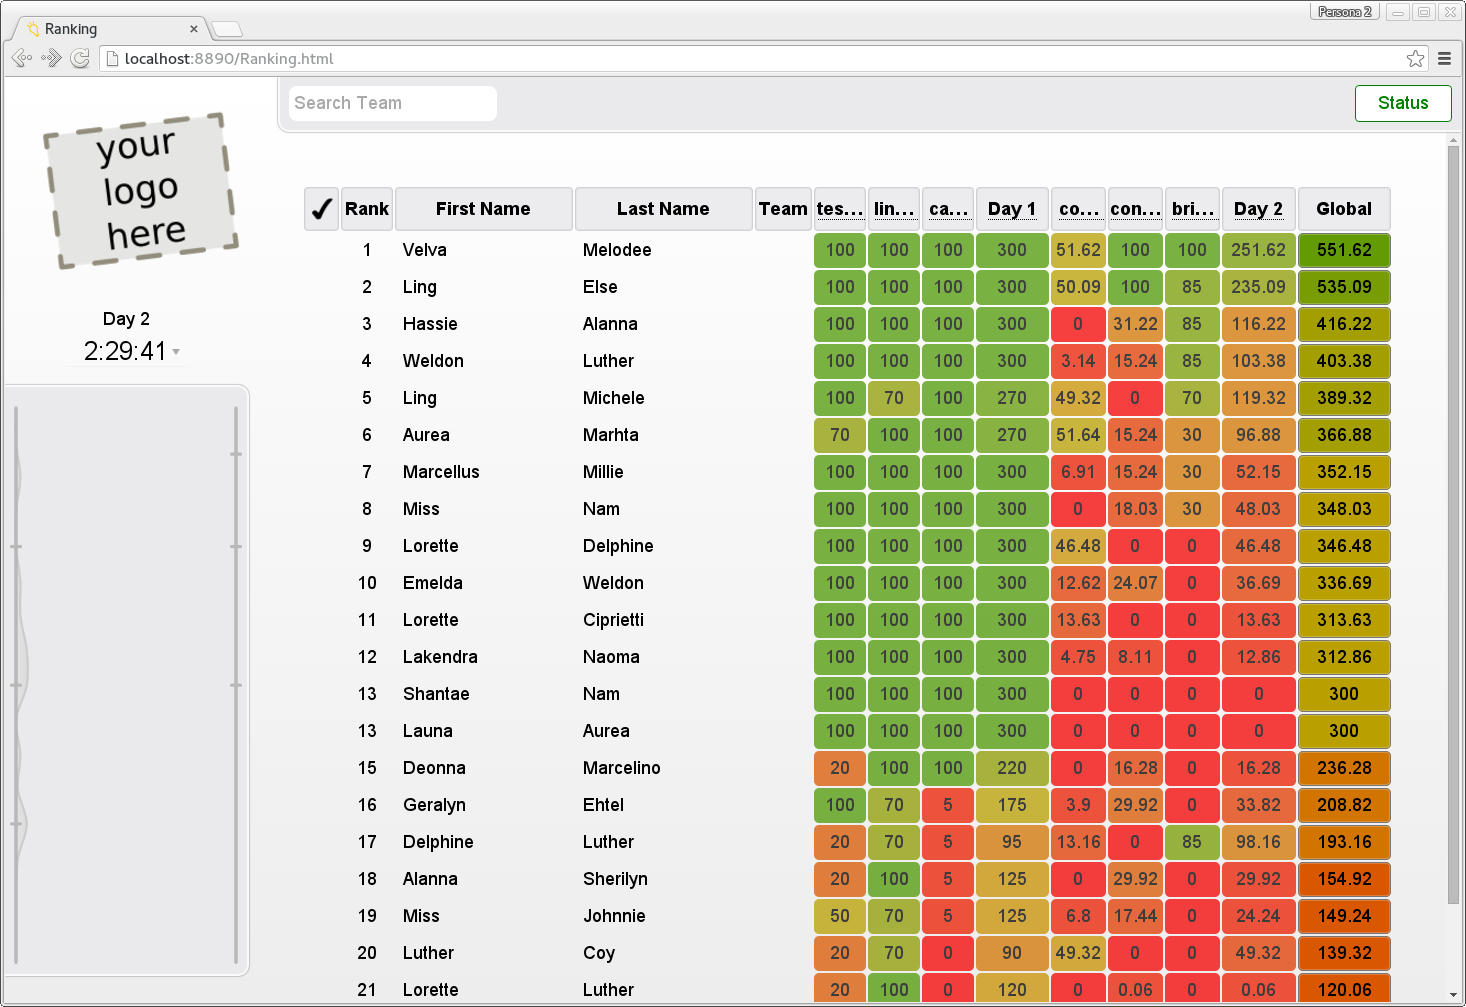
\includegraphics[scale=0.3,trim=4 4 4 4,clip]{Figures/cmsranking.png}
  \caption[Οθόνη βαθμολογιών CMS]{Η οθόνη της βαθμολογίας, με τη συνολική κατάταξη
  και ανά διαγωνιζόμενο σε όλα τα προβλήματα. Πηγή: https://cms-dev.github.io/screenshots.html}
\end{figure}

\begin{figure}
  \centering
  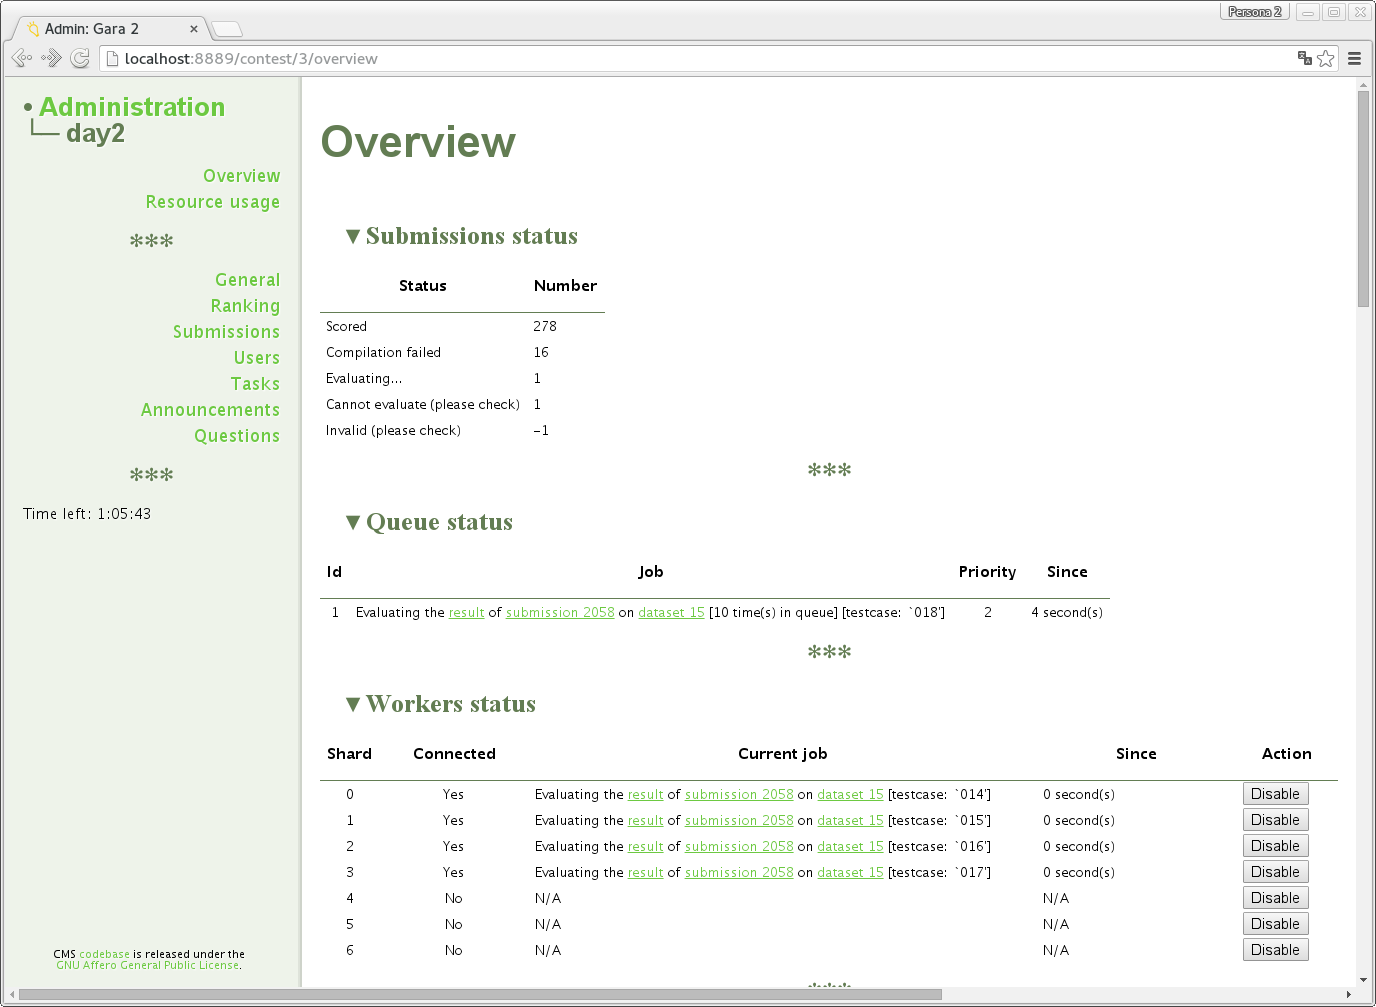
\includegraphics[scale=0.3,trim=4 4 4 4,clip]{Figures/cmsadmin.png}
  \caption[Οθόνη διαχείρισης διαγωνισμού CMS]{Η οθόνη της διαχείρισης ενός
  διαγωνισμού.  Διακρίνονται συνολικά στατιστικά για τις υποβολές, η κατάσταση
  της ουράς και των Workers. Πηγή: https://cms-dev.github.io/screenshots.html}
\end{figure}

\FloatBarrier

\section{Mooshak 2.0}

Το Mooshak 2.0 είναι κι αυτό ένα σύστημα διαχείρισης διαγωνισμών με αυτόματη
αξιολόγηση για τις υποβολές. Αποτελεί τη νεότερη υλοποίηση του Mooshak, με μεταφορά
του κώδικά από C++ και Tcl σε Java με χρήση της εργαλειοθήκης Google Web Toolkit.
H αρχική έκδοση του Mooshak δημιουργήθηκε το 2000 και βασίζεται σε ένα παλαιότερο
διαδικτυακό σύστημα εκμάθησης, το Ganesh. Ο κώδικας του διατίθεται επίσης ελεύθερα
με χρήση της άδειας Artistic License, η οποία δεν προϋποθέτει την διατήρηση
άδειας ελεύθερου λογισμικού σε μελλοντική τροποποίηση και διανομή.

\bigskip

Οι βασικές του προδιαγραφές βασίζονται στους κανόνες των διαγωνισμών ICPC, αλλά
υποστηρίζει και άλλες μορφές διαγωνισμών, όπως είναι οι Ολυμπιάδες πληροφορικής.
Έχει χρησιμοποιηθεί σε πληθώρα τοπικών και διεθνών διαγωνισμών αλλά και σταθερά
στο πλαίσιο εκμάθησης και αξιολόγησης φοιτητών.

\subsection{Τεχνικά Χαρακτηριστικά}

Το Mooshak 2.0 βασίζεται σε μια κοινή αρχιτεκτονική εξυπηρετητή και πελατών με τη
διαφορά ότι υποστηρίζει τη δημιουργία πρόσθετων κόμβων. Οι κόμβοι αυτοί έχουν σκοπό
τη διατήρηση της σταθερότητας και απαιτούν συνεχή συγχρονισμό με τον κεντρικό
εξυπηρετητή ώστε να αναλαμβάνουν μέρος του δικτυακού φόρτου αλλά και να αποτελούν
εφεδρικές λύσεις σε περίπτωση βλάβης των υπολοίπων κόμβων.

\bigskip

\begin{figure}
  \centering
  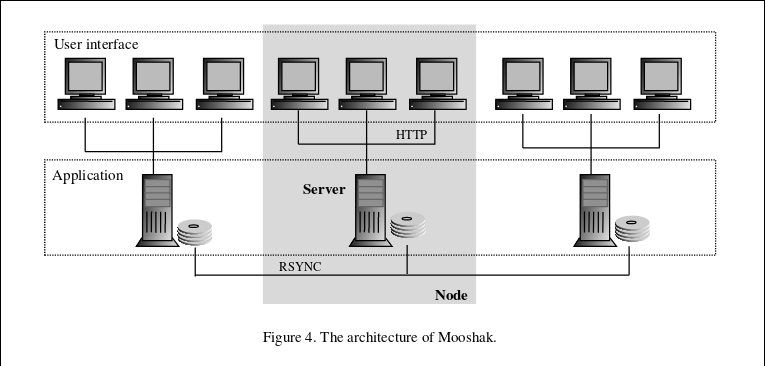
\includegraphics[scale=0.4,trim=4 4 4 4,clip]{Figures/mooshakarchitecture.png}
  \caption[Η αρχιτεκτονική του Mooshak]{Η αρχιτεκτονική του Mooshak με τρεις
  εξυπηρετητές, όπου οι δύο βρίσκονται στο ίδιο τοπικό δίκτυο και όλοι
  συγχρονίζουν τα δεδομένα τους. Βασισμένο στο σχήμα 4 του
  \cite{leal2003mooshak}.}
\end{figure}

\bigskip

Αντίθετα με άλλα συστήματα, το Mooshak δε χρησιμοποιεί βάση και περιορίζεται
στην αποθήκευση όλων των δεδομένων του στο σύστημα αρχείων. Οι γλώσσες
προγραμματισμού που υποστηρίζει περιλαμβάνουν τις C, C++, Java, Pascal, Perl,
Python, Haskell, Haskell και Prolog, ενώ η επέκταση του ώστε να υποστηρίξει
πρόσθετες γλώσσες δεν αποτελεί δύσκολη διαδικασία.

\bigskip

Το σύστημα είναι επίσης παραμετροποιήσιμο ως προς τον τρόπο αξιολόγησης καθώς
έχει σχεδιαστεί για πολλούς διαφορετικούς τύπους διαγωνισμών. Χαρακτηριστικό
είναι ότι στη διαδικασία της υποβολής, πριν από τα στάδια της μεταγλώττισης,
της εκτέλεσης και της αξιολόγησης, δίνεται η δυνατότητα προσθήκης μιας
λειτουργίας στατικής ανάλυσης του πηγαίου κώδικα της υποβολής και αξιολόγησης
του με χρήση κριτηρίων ορισμένων από τους διαχειριστές του διαγωνισμού. Αυτό
επιτρέπει τη χρήση του Mooshak, παραδείγματος χάρη για ένα διαγωνισμό τύπου
code golf, δηλαδή επίτευξης της λύσης με το λιγότερο κώδικα.

\subsection{Εγκατάσταση και Χρήση}

Η εγκατάσταση του Mooshak 2 δεν έχει πολλές απαιτήσεις. Συγκεκριμένα,
χρειάζεται μόνο το περιβάλλον της Java και το λογισμικό του εξυπηρετητή. Σε
αυτό το σημείο, μπορούν να στηθούν επίσης επιπλέον κόμβοι εάν είναι επιθυμητό,
τοπικά ή απομακρυσμένα. Μόλις στηθεί το σύστημα, η δημιουργία των διαγωνισμών
και των προβλημάτων γίνεται μέσω της δικτυακής διεπαφής του Διαχειριστή.

\bigskip

Οι διαγωνιζόμενοι, μπαίνοντας στην ιστοσελίδα του Mooshak, μπορούν να διαβάσουν
τις περιγραφές των προβλημάτων και να πραγματοποιήσουν τις υποβολές τους είτε
ανεβάζοντας το πρόγραμμα τους, είτε χρησιμοποιώντας τον επεξεργαστή κειμένου της
ιστοσελίδας ώστε να το συντάξουν επιτόπου.

\bigskip

Οι δημιουργοί του Mooshak παραθέτουν στη σελίδα του μόνιμα περιβάλλοντα δοκιμών,
στα οποία μπορεί ο οποιοσδήποτε να χρησιμοποιήσει ένα ζωντανό Mooshak σύστημα είτε
για να πραγματοποιήσει υποβολές, είτε για να δημιουργήσει νέους διαγωνισμούς και
προβλήματα.

\bigskip

\begin{figure}
  \centering
  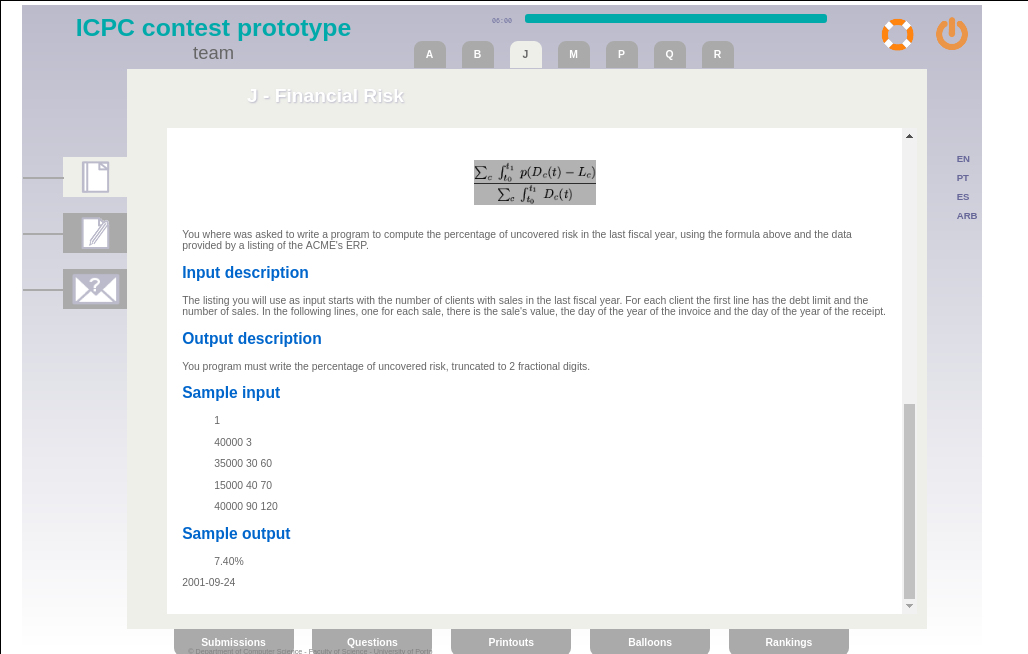
\includegraphics[scale=0.3,trim=4 4 4 4,clip]{Figures/mooshakproblem.png}
  \caption[Οθόνη δ]{Η οθόνη της διαχείρισης ενός διαγωνισμού.
  Διακρίνονται συνολικά στατιστικά για τις υποβολές, η κατάσταση της ουράς και των
  Workers.}
\end{figure}

\begin{figure}
  \centering
  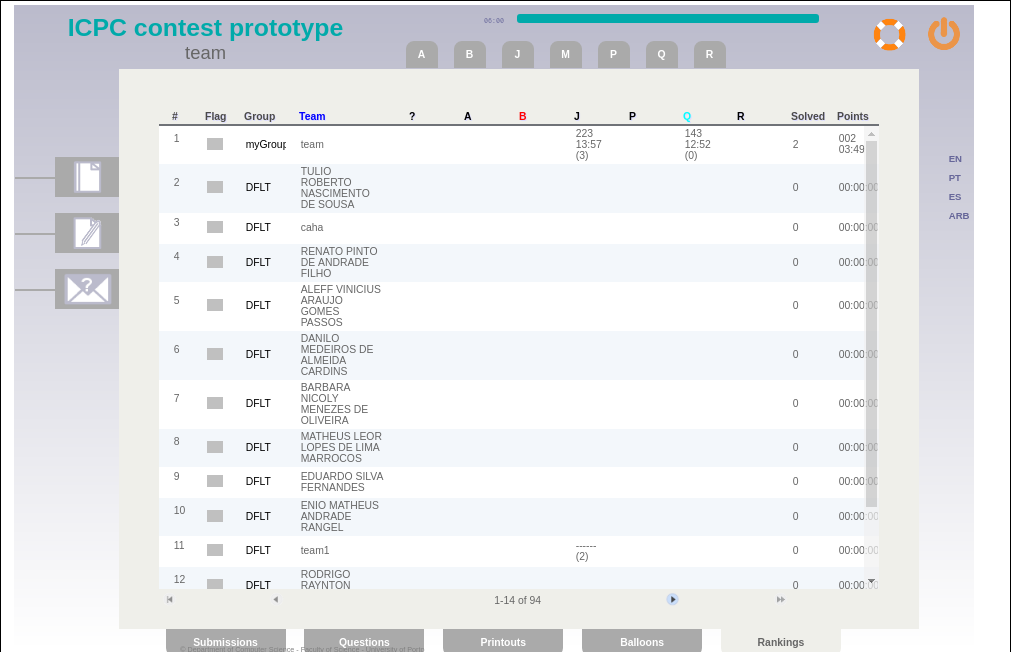
\includegraphics[scale=0.3,trim=4 4 4 4,clip]{Figures/mooshakrankings.png}
  \caption[Οθόνη διαχείρισης προβλήματος]{Η οθόνη της διαχείρισης ενός διαγωνισμού.
  Διακρίνονται συνολικά στατιστικά για τις υποβολές, η κατάσταση της ουράς και των
  Workers.}
\end{figure}

\FloatBarrier

\section{CATS}

To CATS είναι το τρίτο σύστημα που θα αναλυθεί. Αφορά και αυτό τη διεξαγωγή και
τον έλεγχο προγραμματιστικών διαγωνισμών και συντηρείται από τον Alexander Klenin
του Far Eastern Federal University. Χρησιμοποιείται τόσο για μεγάλες διοργανώσεις,
όπως είναι το ICPC Ρωσίας και Άπω Ανατολής, καθώς και για πλήθος ακαδημαϊκών
μαθημάτων και διαγωνισμών. Κατέχει άδεια GPL 2.0 επιτρέποντας την ελεύθερη
χρήση, τροποποίηση και διανομή του.

\bigskip

Έχει αρκετές δυνατότητες που το διακρίνουν ανάμεσα στα υπόλοιπα συστήματα
συμπεριλαμβανομένων των παρακάτω:

\begin{itemize}
    \item Μεγάλος αριθμός προγραμματιστικών γλωσσών και μεταγλωττιστών
    \item Αυτόματος ορισμός διαγωνισμών, προβλημάτων και αρχείων ελέγχου με χρήση
      ενός zip αρχείου με μια περιγραφή σε XML
    \item Έτοιμα πρόσθετα (modules) για την αξιολόγηση των υποβολών, π.χ. για
      αυτόματη δημιουργία αρχείων ελέγχου
    \item Περιορισμός πρόσβασης ανάλογα με τη διεύθυνση IP των χρηστών
    \item Αυτόματος έλεγχος για αντιγραφή κώδικα μεταξύ των διαγωνιζομένων
\end{itemize}

\subsection{Τεχνικά Χαρακτηριστικά}

Το CATS είναι υλοποιημένο σε Perl και χρησιμοποιεί βάση δεδομένων Oracle. Το
σύστημα αποτελείται από τον εξυπηρετητή που "σηκώνει" την ιστοσελίδα του
διαγωνισμού για διαγωνιζόμενους και διαχειριστές και από τον εξυπηρετητή των
αξιολογήσεων, ο οποίος αναλαμβάνει τη δημιουργία των δυνητικά επικίνδυνων
εργασιών που τρέχουν σε ένα περιορισμένο περιβάλλον με τη χρήση ενός πρόσθετου
που λέγεται spawner.

\bigskip

Η εφαρμογή αξιολόγησης εμπεριέχει διεπαφή μέσω της γραμμής εντολών για τη
γρήγορη δημιουργία και αξιολόγηση προβλημάτων από τους διαχειριστές. Αυτή
διατίθεται και ανεξάρτητα από το υπόλοιπο πρόγραμμα προς αντικατάσταση
αντίστοιχων διαδικτυακών εργαλείων όπως είναι το Polygon
\footnote{https://polygon.codeforces.com/}. Η δημιουργία των προβλημάτων
γίνεται με το ανέβασμα ενός συμπιεσμένου αρχείου το οποίο περιέχει μια XML
περιγραφή και τα απαραίτητα αρχεία ελέγχου.

\lstinputlisting[caption=Παράδειγμα xml]{Listings/catsexample.xml}

\bigskip

Οι γλώσσες προγραμματισμού που υποστηρίζονται είναι οι C, C++, delphi, VB, Java,
C\#, Perl, Python, Ruby, PHP, Erlang, Javascript και SQL.

%TODO mipws valw kai ta site twn sistimatwn
%TODO paper rozhkov
\subsection{Εγκατάσταση και Χρήση}

Η εγκατάσταση του CATS είναι αρκετά εύκολη, καθώς έχει πολύ λίγες εξαρτήσεις
και διαθέτει έτοιμα scripts για το deployment και την αρχική παραμετροποίηση.
Αφού τρέξουν αυτά και ρυθμιστεί η σύνδεση με τη βάση, το σύστημα είναι έτοιμο
να χρησιμοποιηθεί.

\bigskip

Η διαδικασία εμφάνισης των ορισμών των προβλημάτων, υποβολής των λύσεων και
διαχείρισης των διαγωνισμών από τους διαχειριστές είναι παρόμοια με τα προηγούμενα
συστήματα και παρουσιάζεται με φωτογραφίες παρακάτω. Είναι ενδιαφέρουσα και χρήσιμη
η δυνατότητα του CATS για διαχείριση διαγωνισμών, αξιολόγηση και παρουσίαση των
αποτελεσμάτων απ᾽ευθείας μέσω της γραμμής εντολών μέσω του API που προσφέρεται.

\begin{figure}
  \centering
  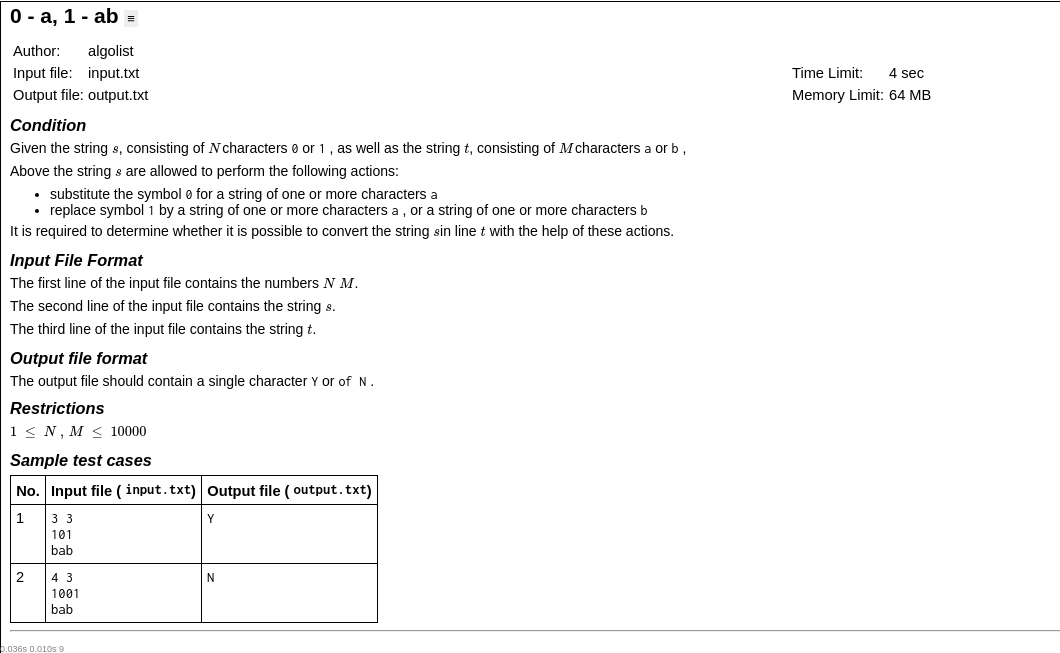
\includegraphics[scale=0.3,trim=4 4 4 4,clip]{Figures/catsproblem.png}
  \caption[Οθόνη διαχείρισης προβλήματος]{Η οθόνη της διαχείρισης ενός διαγωνισμού.
  Διακρίνονται συνολικά στατιστικά για τις υποβολές, η κατάσταση της ουράς και των
  Workers.}
\end{figure}

\begin{figure}
  \centering
  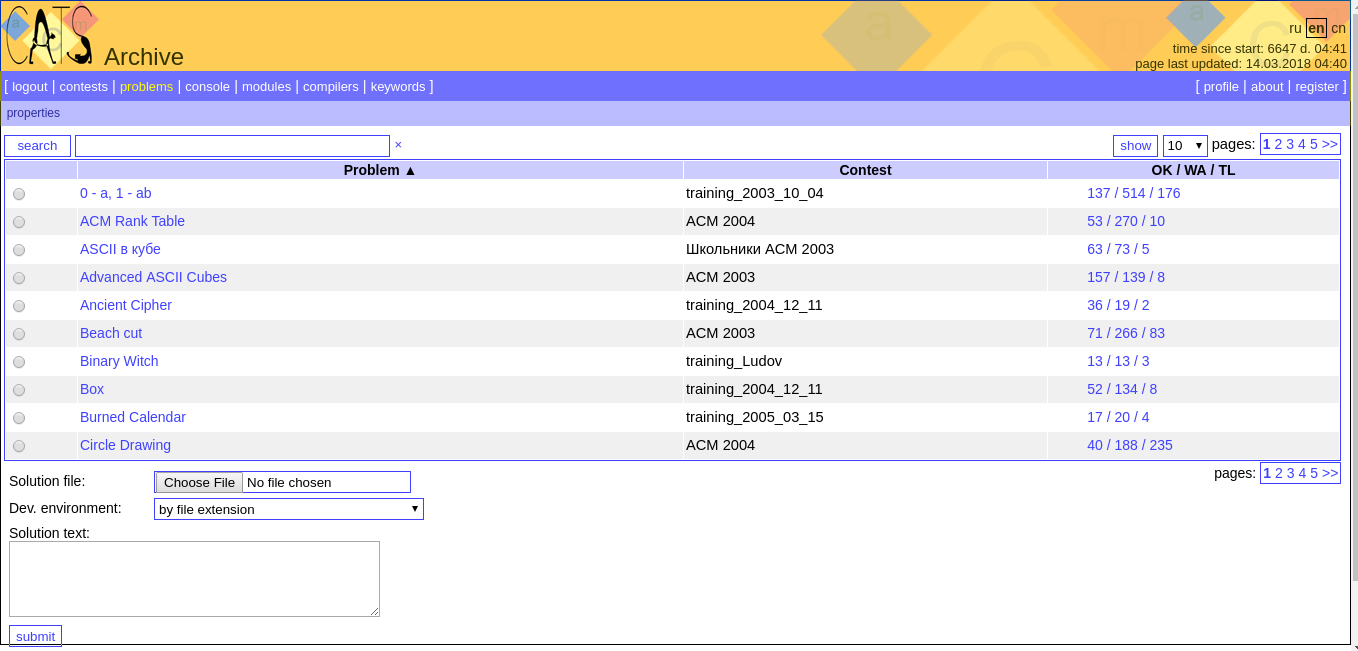
\includegraphics[scale=0.3,trim=4 4 4 4,clip]{Figures/catssubmission.png}
  \caption[Οθόνη διαχείρισης προβλήματος]{Η οθόνη της διαχείρισης ενός διαγωνισμού.
  Διακρίνονται συνολικά στατιστικά για τις υποβολές, η κατάσταση της ουράς και των
  Workers.}
\end{figure}

\FloatBarrier

\chapter{Περιγραφή Grader - Kewii}

Το σύστημα αποτελείται από το το σύστημα αξιολόγησης Kewii, το backend της
εφαρμογής μας που λειτουργεί ως δαίμονας στον εξυπηρετητή με σκοπό την
μεταγλώττιση και αξιολόγηση των υποβολών που λαμβάνει, και από τη διαδικτυακή
εφαρμογή Grader, η οποία αναλαμβάνει την αλληλεπίδραση με χρήστες και
διαχειριστές, την (έμμεση) επικοινωνία με τον Kewii και τη συνολική υλοποίηση
της λογικής του συστήματος όσον αφορά στον τρόπο λειτουργίας των επιμέρους
στοιχείων του και τον τρόπο αξιολόγησης.

\section{Στοιχεία και έννοιες του συστήματος}

Στην ενότητα αυτή θα περιγραφούν συνοπτικά τα συστατικά στοιχεία του συστήματος
μας. Η γνώση τους είναι απαραίτητη για να γίνει αντιληπτός ο διαχωρισμός μεταξύ
Kewii και Grader, δηλαδή backend και frontend.

\subsection{Προβλήματα}

Προβλήματα είναι οι ανεξάρτητες ασκήσεις που τίθενται προς επίλυση στους
διαγωνιζόμενους/χρήστες. Κάθε πρόβλημα έχει χρονικά όρια εκτέλεσης και όρια
μνήμης, όπως και ιδιότητες για τον τρόπο εκτέλεσης και αξιολόγησης. Η
αξιολόγηση του γίνεται πάνω σε συγκεκριμένα αρχεία εισόδου και εξόδου, τα
αρχεία ελέγχου. Προαιρετικά, ένα πρόβλημα μπορεί, επιπλέον, να διαθέτει ένα
πρόγραμμα αξιολόγησης των υποβολών.

\bigskip

Τα προβλήματα έχουν νόημα μόνο μέσα σε διαγωνισμούς, καθώς ο διαγωνιζόμενος
παίρνει μέρος σε διαγωνισμούς που περιέχουν προβλήματα και η τελική βαθμολογία
του είναι το άθροισμα των επιδόσεων του στα προβλήματα του διαγωνισμού. Η
αρχική σχεδίαση του συστήματος είχε ως στόχο τη χρήση αυτού σε διαγωνισμούς
πληροφορικής, οπότε τα προβλήματα είναι συνδεδεμένα στενά τόσο με τον
διαγωνισμό που ανήκουν όσο και με τις υποβολές που έχουν γίνει σε αυτά. Κάθε
πρόβλημα μπορεί να ανήκει μόνο σε ένα διαγωνισμό.

\bigskip

Σε επόμενο κεφάλαιο θα διερευνηθεί και θα περιγραφεί η υλοποίηση ενός εναλλακτικού
σχεδιασμού που επιτρέπει την χρήση των προβλημάτων σε διάφορους διαγωνισμούς και
την αλλαγή της σύνδεσης των υποβολών από το πρόβλημα προς τους διαγωνισμούς.

\subsection{Διαγωνισμοί}

Οι διαγωνισμοί αντιστοιχούν σε πραγματικούς διαγωνισμούς, εξετάσεις ή σειρές
ασκήσεων. Εμπεριέχουν προβλήματα και είναι ενεργοί/ορατοί σε ένα χρονικό
διάστημα όπου οι διαγωνιζόμενοι μπορούν να υποβάλλουν τις λύσεις τους. Μόλις
ολοκληρωθεί η διεξαγωγή τους, ο διαχειριστής μπορεί να εκκινήσει την τελική
αξιολόγηση, κατά την οποία βαθμολογούνται οι ενεργές υποβολές των
διαγωνιζόμενων σε όλα τα προβλήματα του διαγωνισμού. Οι διαγωνισμοί μπορούν να
είναι ορατοί μόνο από επιλεγμένους χρήστες ή από όλους.

\subsection{Αρχεία Ελέγχου}

Τα αρχεία ελέγχου είναι ζευγάρια αρχείων εισόδου και εξόδου και ανήκουν σε
προβλήματα. Μια σωστή υποβολή/λύση θα πρέπει για κάθε αρχείο εισόδου
που δέχεται, να παράγει έξοδο ίδια με αυτή του αντίστοιχου αρχείο εξόδου.
Κάθε αρχείο ελέγχου χαρακτηρίζεται από τον τύπο του, αναφορικά με το πότε
εκτελείται και αν είναι ορατό στους χρήστες. Οι τύποι εκτέλεσης αντιστοιχούν
σε χρώματα (tags) και παρουσιάζονται στον Πίνακα 3.1.

  \begin{table}
    \begin{tabular}{ | l | p{10cm} |}
    \hline
    Τύπος εκτέλεσης & Λειτουργία \\ \hline
    Πορτοκαλί 
\includegraphics[scale=0.8]{Figures/tag_orange.png} &
      Το αρχείο ελέγχου χρησιμοποιείται σε κάθε υποβολή για το συγκεκριμένο πρόβλημα
      αλλά δεν είναι ορατό στους χρήστες. \\ \hline
    Κίτρινο 
\includegraphics[scale=0.8]{Figures/tag_yellow.png} &
      Το αρχείο ελέγχου χρησιμοποιείται σε κάθε υποβολή για το συγκεκριμένο πρόβλημα
      και είναι ορατό στους χρήστες. \\ \hline
    Πράσινο 
\includegraphics[scale=0.8]{Figures/tag_green.png} &
      Το αρχείο ελέγχου χρησιμοποιείται μόνο κατά την τελική αξιολόγηση. \\ \hline
    Μωβ 
\includegraphics[scale=0.8]{Figures/tag_purple.png} &
      Το αρχείο ελέγχου δεν χρησιμοποιείται. \\ \hline
    \end{tabular}
  \caption{Τύποι εκτέλεσης αρχείων ελέγχου}
  \end{table}

\bigskip

Σε επόμενο κεφάλαιο θα δημιουργηθεί άλλος ένας τύπος εκτέλεσης. Επιπλέον, θα
αλλάξει ριζικά ο τρόπος αξιολόγησης καθώς θα εισαχθεί η έννοια των ομάδων
αρχείων ελέγχου και τα αρχεία θα έχουν νόημα μόνο μέσα σε αυτές.

\subsection{Χρήστες/Διαγωνιζόμενοι}

Οι χρήστες ή διαγωνιζόμενοι είναι τα άτομα που αλληλεπιδρούν με το σύστημα με
σκοπό την υποβολή λύσεων στους διαγωνισμούς που συμμετέχουν. Οι διαχειριστές
αποτελούν κι αυτοί χρήστες, με τη διαφορά ότι έχουν δικαίωμα πρόσβασης στις
σελίδες διαχείρισης διαγωνισμών και προβλημάτων. Οι τελευταίοι έχουν επίσης
δικαίωμα να εισάγουν νέους χρήστες από ένα αρχείο, να ορίσουν την ορατότητα των
διαγωνισμών για συγκεκριμένους διαγωνιζόμενους και να απαντήσουν σε μηνύματα
αυτών.

\subsection{Υποβολές}

Η υποβολή μιας λύσης εμπεριέχει το "ανέβασμα" του κώδικα του διαγωνιζόμενου για
να γίνει η μεταγλώττιση του στον εξυπηρετητή, να εκτελεστεί από τον Kewii για
κάθε αρχείο ελέγχου που αντιστοιχεί στο είδος της υποβολής και να αξιολογηθεί η
ορθότητα της εξόδου. Οι υποβολές χωρίζονται σε δύο κύριες κατηγορίες, την
κανονική και την τελική. Ουσιαστικά, όλες οι υποβολές των διαγωνιζόμενων είναι
κανονικές και εφόσον υπάρχει, για έναν διαγωνιζόμενο, τουλάχιστον μία υποβολή
που περνάει όλα τα αρχεία ελέγχου στα οποία αξιολογήθηκε, αυτή θεωρείται ενεργή
για αυτόν. Όταν ολοκληρωθεί η περίοδος ανοιχτών υποβολών ενός διαγωνισμού, όλες
οι ενεργές υποβολές για κάθε πρόβλημα του διαγωνισμού επαναυποβάλλονται για την
τελική αξιολόγηση τους.

\subsection{Προγράμματα Αξιολόγησης}

Οι υποβολές σε κάθε πρόβλημα αξιολογούνται με σύγκριση της εξόδου του υποβληθέντος
προγράμματος με αυτήν του αρχείου ελέγχου για την αντίστοιχη είσοδο. Εξαίρεση σε
αυτό τον τρόπο αξιολόγησης, αποτελούν τα προβλήματα που διαθέτουν το δικό τους
πρόγραμμα αξιολόγησης το οποίο αναλαμβάνει να συγκρίνει την αναμενόμενη έξοδο
με αυτήν που παρήγαγε το υποβληθέν πρόγραμμα και να βαθμολογήσει αυτή την έξοδο
στην κλίμακα [0, 1]. Το πρόγραμμα αξιολόγησης είναι και αυτό αποθηκευμένο στον
εξυπηρετητή και μεταγλωττίζεται και εκτελείται από τον Kewii.


\section{Σύστημα αξιολόγησης Kewii}

Ο Kewii είναι μια εφαρμογή γραμμένη σε γλώσσα C και τρέχει στον εξυπηρετητή
ελέγχοντας διαρκώς για νέες υποβολές. Για κάθε νέα υποβολή που εντοπίζει,
βρίσκει τον πηγαίο κώδικα που έχει αποθηκευτεί από τον Grader μαζί με συγκεκριμένα
μεταδεδομένα, μεταγλωττίζει τον κώδικα δημιουργώντας το εκτελέσιμο αρχείο και το
εκτελεί χρησιμοποιώντας τα απαραίτητα μέτρα ασφαλείας ώστε να συγκρίνει την έξοδο
για κάθε αρχείο ελέγχου με την σωστή. Μόλις τελειώσει η εκτέλεση ή ξεπεραστούν τα
όρια της, ενημερώνει τη βάση δεδομένων, με χρήση ενός PHP script, με την έκβαση της
εκτέλεσης και ειδοποιεί το Grader καλώντας ένα μοναδικό για κάθε υποβολή σύνδεσμο
(callback) ώστε αυτός να αναλάβει την ανάλυση των αποτελεσμάτων.

\bigskip

Κάθε υποβολή έχει έναν μοναδικό κωδικό, ο οποίος χρησιμοποιείται για την
αλληλεπίδραση με το Grader κατά το callback, όπως και έναν αύξοντα αριθμό που
χρησιμεύει στον Kewii για την διατήρηση της κατάστασης των εκτελέσεων. Τα
μεταδεδομένα που εμπεριέχονται σε κάθε υποβολή και είναι απαραίτητα για την
αξιολόγηση της είναι τα παρακάτω:

\begin{itemize}
  \item Όνομα του προβλήματος
  \item Γλώσσα υποβολής
  \item Αρχεία ελέγχου που θα χρησιμοποιηθούν
  \item Όριο μνήμης και χρόνου εκτέλεσης
  \item Είδος εκτέλεσης
  \item Τρόπος αξιολόγησης
\end{itemize}

Κάθε πρόβλημα πρέπει να έχει μοναδικό όνομα και είναι απαραίτητο ώστε να
επιλεχθούν τα σωστά αρχεία ελέγχου. Οι γλώσσες υποβολής που υποστηρίζονται
είναι: C, C++, Pascal, Pazcal, F\#, OCaml, SML, Java, Fortran και Haskell. Το
είδος εκτέλεσης μπορεί να είναι batch ή interactive/partial. Στην πρώτη
περίπτωση τα προγράμματα που υποβάλλονται αποτελούν ανεξάρτητες λύσεις ενώ στην
δεύτερη ο κώδικάς αλληλεπιδρά με συγκεκριμένες βιβλιοθήκες ή εντάσσεται σε έναν
κοινό κορμό που έχει τεθεί για το συγκεκριμένο πρόβλημα. Ο τρόπος αξιολόγησης
μπορεί να είναι κανονικός ή ειδικός. Στον κανονικό ελέγχεται η ομοιότητα της
εξόδου του προγράμματος της υποβολής με την ορθή απάντηση, ενώ στον ειδική
αξιολόγηση γίνεται χρήση ενός προγράμματος, που θα έχει τεθεί για το
συγκεκριμένο πρόβλημα, ώστε να βαθμολογηθεί η λύση, επιτρέποντας έτσι την
ύπαρξη προβλημάτων βελτιστοποίησης.

\bigskip

Οι υποβολές που στέλνονται στον Kewii αποθηκεύονται σε μια ουρά σύμφωνα με τον
αύξοντα αριθμό που παίρνουν και ο Kewii γνωρίζει κάθε στιγμή ποιος θα είναι ο
επόμενος αριθμός υποβολής που θα αξιολογήσει. Το πρόγραμμα κοιμάται έως ότου
βρει μια νέα υποβολή ελέγχοντας για αρχεία με τον συγκεκριμένο αριθμό. Επίσης,
αν η διαδικασία της αξιολόγησης διακοπεί ενδιάμεσα, μπορεί να συνεχίσει από το
σημείο που σταμάτησε. Μια ακριβέστερη περιγραφή της ροής φαίνεται στο παρακάτω
σχήμα:

\begin{figure}
  \centering
  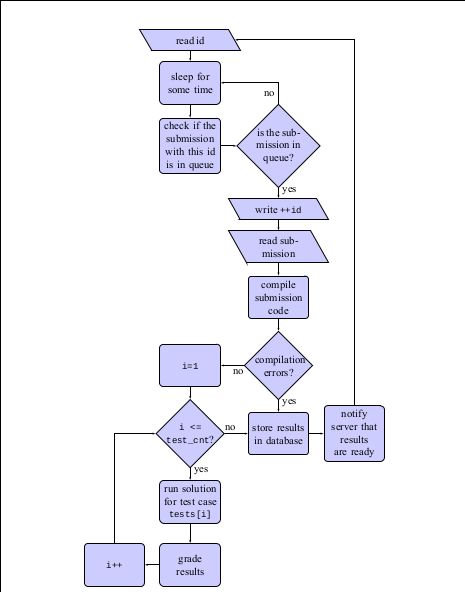
\includegraphics[scale=0.3,trim=4 4 4 4,clip]{Figures/graderflow.png}
  \caption[Οθόνη διαχείρισης προβλήματος]{Η οθόνη της διαχείρισης ενός διαγωνισμού.
  Διακρίνονται συνολικά στατιστικά για τις υποβολές, η κατάσταση της ουράς και των
  Workers.}
\end{figure}

\bigskip

Γενικά, ο Kewii περιορίζεται στο να δέχεται υποβολές για συγκεκριμένα προβλήματα
με συγκεκριμένα αρχεία ελέγχου (και σε μερικές περιπτώσεις συγκεκριμένο πρόγραμμα
αξιολόγησης). Αξιολογεί την κάθε υποβολή με 0 - λάθος και 1 - σωστό για κάθε αρχείο
ή αναθέτει την αξιολόγηση στο αρμόδιο πρόγραμμα που θα επιστρέψει μια τιμή ανάμεσα
στα 0 και 1. Τότε οι "ευθύνες" του τελειώνουν, δηλαδή δεν ασχολείται με την συνολική
αξιολόγηση των διαγωνισμών και των προβλημάτων και ποια υποβολή θεωρείται ενεργή,
ούτε με το ποια αρχεία ελέγχου θα επιλεγούν κατά την υποβολή. Τα παραπάνω κρίνονται
σημαντικά γιατί θα μας επιτρέψουν να επανασχεδιάσουμε τον αλγόριθμο της υποβολής,
δημιουργώντας ομάδες αρχείων ελέγχου, όπως και άλλα κομμάτια του Grader χωρίς να
χρειαστεί να τροποποιήσουμε τον Kewii.

\section{Διαδικτυακή εφαρμογή Grader}

Ο Grader είναι μια web εφαρμογή υλοποιημένη σε PHP και HTML/CSS/JS, η οποία
αποτελεί το frontend και μέρος του backend του συστήματος μας. Ως frontend
εφαρμογή αναλαμβάνει να παρουσιάσει σε διαγωνιζόμενους και διαχειριστές τις
σελίδες διαχείρισης, υποβολών και αποτελεσμάτων, ενώ ως backend αναλαμβάνει την
υλοποίηση της λογικής του συστήματος, των διάφορων αλγορίθμων και ροών και την
επικοινωνία με τη βάση δεδομένων και τον Kewii.

\bigskip

\noindent Τα συνήθη σενάρια χρήσης της εφαρμογής αναφέρονται παρακάτω.

\subsection{Εμφάνιση διαθέσιμων διαγωνισμών και προβλημάτων}

Τόσο οι διαγωνιζόμενοι, όσο και οι διαχειριστές έχουν τη δυνατότητα να βλέπουν
τους ενεργούς διαγωνισμούς και τα προβλήματα που περιέχονται σε αυτούς. Η
σελίδα κάθε διαγωνισμού ενημερώνει το χρήστη για τη διάρκεια του καθώς και για
το ποια προβλήματα περιέχει. Μεταβαίνοντας σε κάποιο πρόβλημα, ο χρήστης βλέπει
την ακριβή περιγραφή του και έχει τη δυνατότητα να υποβάλλει τη λύση του.

\subsection{Εμφάνιση υποβολών προβλήματος και πηγαίου κώδικα}

Κάθε χρήστης μπορεί μέσα από τη σελίδα του διαγωνισμού να περάσει στις υποβολές
για καθένα από τα προβλήματα του. Σε αυτή τη σελίδα υπάρχουν όλες οι υποβολές
που έχει κάνει για αυτό το πρόβλημα, ενώ υπάρχει χρωματική διάκριση ανάμεσα σε
σωστές και λανθασμένες υποβολές, καθώς και για την ενεργή υποβολή. Ως ενεργή
υποβολή τίθεται η τελευταία σωστή, αν και υπάρχει η δυνατότητα, στην ίδια
οθόνη, να επιλεχθεί μια διαφορετική σωστή υποβολή ως ενεργή. Επιλέγοντας μια
υποβολή, ο χρήστης μεταφέρεται στην οθόνη λεπτομερειών της υποβολής του, όπου
εμφανίζονται και τα ακριβή αποτελέσματα της λύσης του για κάθε αρχείο ελέγχου.
Για τα αρχεία ελέγχου που το επιτρέπουν, υπάρχει η οθόνη προεπισκόπησης.
Παρόμοια δυνατότητα δίνεται και για τον πηγαίο κώδικα της υποβολής, αν ο
χρήστης θέλει να τον δει στην εφαρμογή.

TODO: μιλαμε για σεναρια οχι για οθονες, μηπως θελουν αλλαγη οι περιγραφες;
\subsection{Δημιουργία και διαχείριση προβλημάτων και διαγωνισμών}

Στη συγκεκριμένη οθόνη, που δεν είναι προσβάσιμη στους κανονικούς χρήστες, ο
διαχειριστής μπορεί να δει όλους τους διαγωνισμούς και τα προβλήματα που έχουν
δημιουργηθεί. Οι διαγωνισμοί παρουσιάζονται ταξινομημένοι κατά χρονολογική
σειρά δημιουργίας μαζί με τα προβλήματα που περιέχονται στον καθένα. Δίνονται
επιλογές για επεξεργασία προβλημάτων και διαγωνισμών, καθώς και δημιουργία
νέων. Αφού δημιουργηθεί ένα πρόβλημα, αρχικά δεν ανήκει σε κάποιον διαγωνισμό
έως ότου επιλεχθεί κάποιος από το πλευρικό μενού μετακίνησης του προβλήματος.
Διπλά σε κάθε πρόβλημα υπάρχουν, επιπλέον, στοιχεία για τα αρχεία ελέγχου που
διαθέτει και τις συνολικές λύσεις που έχουν υποβληθεί.

\bigskip

Εξαιτίας της άμεσης σύνδεσης προβλημάτων και υποβολών σε αυτά, κατά τη
μετακίνηση ενός προβλήματος μεταξύ διαγωνισμών, αυτό διατηρεί τις υποβολές που
είχε αν και είναι πλέον σε διαφορετικό διαγωνισμό. Επιπροσθέτως, όπως είναι
προφανές, ο διαγωνισμός που ήταν αρχικά το πρόβλημα φαίνεται κενός και
ουσιαστικά χάνει και την ιστορικότητα του. Ο συγκεκριμένος τρόπος λειτουργίας
αποτελεί απόρροια της αρχικής σχεδίασης του Grader για διοργανώσεις και όχι για
ακαδημαϊκούς σκοπούς, με αποτέλεσμα να μην έχει προβλεφθεί η δημιουργία
διαγωνισμών-σειρών ασκήσεων με επαναχρησιμοποίηση προβλημάτων.

\bigskip

Μια ακόμα οθόνη που είναι προσβάσιμη από την κεντρική της διαχείρισης προβλημάτων
και διαγωνισμών είναι αυτή των αρχείων ελέγχου του προβλήματος. Σε αυτήν μπορεί
ο διαχειριστής να ανεβάσει καινούρια αρχεία ελέγχου, καθώς και να αλλάξει τον τύπο
εκτέλεσης και την βαθμολογία τους. Η συγκεκριμένη οθόνη θα μας απασχολήσει αρκετά
στα επόμενα κεφάλαια.

\subsection{Ενεργοποίηση διαγωνισμού και τελική αξιολόγηση}

Ένα πολύ συνηθισμένο σενάριο χρήσης για έναν διαχειριστή είναι αυτό κατά το
οποίο, αφού έχει δημιουργήσει ένα νέο διαγωνισμό και τα προβλήματα του, πρέπει
να το δημοσιοποιήσει στους χρήστες. Μέσα από την οθόνη διαχείρισης των
διαγωνισμών, έχει τη δυνατότητα, αρχικά, να επιλέξει τους χρήστες που
επιτρέπεται να συμμετέχουν (ή όλους) στο διαγωνισμό. Έπειτα, έχοντας επιλέξει
και τη σωστή ημερομηνία έναρξης και λήξης του διαγωνισμού κατά τη δημιουργία
του, μπορεί να επιλέξει την ενεργοποίηση αυτού με το αντίστοιχο πλήκτρο στην
οθόνη διαχείρισης. Τότε το πρόβλημα γίνεται ορατό στους επιλεγμένους χρήστες
και οι τελευταίοι μπορούν να ξεκινήσουν να κάνουν υποβολές.

\bigskip

Όταν λήξει ή απενεργοποιηθεί ο διαγωνισμός, ο διαχειριστής μπορεί να εκκινήσει
την τελική αξιολόγηση, κατά την οποία επιλέγονται όλες οι ενεργές υποβολές για
κάθε πρόβλημα του διαγωνισμού (μία ανά διαγωνιζόμενο με τουλάχιστον μία σωστή
υποβολή) και αυτές αποστέλλονται ξανά στον Kewii για να αξιολογηθούν εκ νέου
συμπεριλαμβάνοντας αυτή τη φορά τα αρχεία ελέγχου που είναι αποκλειστικά για
την τελική αξιολόγηση. Μόλις ολοκληρωθεί η διαδικασία, εμφανίζονται στην οθόνη
τα τελικά αποτελέσματα, τα οποία μπορούν να δημοσιοποιηθούν σαν νέα στην αρχική
σελίδα του Grader. Η βαθμολογία υπολογίζεται από το άθροισμα των ενεργών
υποβολών του κάθε διαγωνιζόμενου στα προβλήματα που περιέχει ο διαγωνισμός. Η
βαθμολογία του προβλήματος είναι το άθροισμα των αρχείων ελέγχου της τελικής
αξιολόγησης (αποκλειστικά και μη).

TODO: Καλύτερη περιγραφή της λειτουργίας της υποβολης; + ισως μια συμπερασματική παράγραφο

\chapter{Προσθήκη Ομάδων Αρχείων Ελέγχου}

Η μεγαλύτερη σε πολυπλοκότητα αλλαγή λειτουργικότητας του Grader ήταν η
τροποποίηση του τρόπου αξιολόγησης των υποβολών με την εισαγωγή ομάδων αρχείων
ελέγχου (testcase groups) για ομαδοποίηση των τελευταίων, καθώς και ενός νέου
τύπου εκτέλεσης των αρχείων ελέγχου. Η υλοποίηση του νέου τύπου εκτέλεσης, που
θα αντιστοιχεί στο μπλε χρώμα (blue tag), κατά την αντιστοίχιση που
παρουσιάστηκε στο κεφάλαιο 3.1.3, ήταν μια χρήσιμη εισαγωγή στη
λειτουργία και στο codebase του Grader αλλά και στη βάση και τους σχετικούς
πίνακες. Στο παρόν κεφάλαιο θα περιγραφεί πρώτα η μικρή αυτή προσθήκη και
έπειτα η λογική και η υλοποίηση της προσθήκης των testcase groups.


\section{Προσθήκη blue tag για μη απαραίτητα αρχεία ελέγχου}

\subsection{Κίνητρο}

Ένα αρχείο ελέγχου χαρακτηρισμένο με blue tag, ελέγχεται κανονικά σε κάθε
αξιολόγηση, αλλά το αποτέλεσμα της εκτέλεσης του δεν επηρεάζει την ορθότητα της
υποβολής. Όπως τα "κίτρινα" αρχεία ελέγχου, τα "μπλε", δεν διαθέτουν την είσοδο
τους προς προβολή στους διαγωνιζόμενους. Ο συγκεκριμένος τύπος εκτέλεσης είχε
υλοποιηθεί πρώτα (πριν την παρούσα εργασία), στο branch του Grader που
χρησιμοποιεί το hellenico.gr, το οποίο όμως διαφέρει αρκετά από αυτό του softlab,
γεγονός που δεν επέτρεπε το απλό merge του σχετικού κώδικά.


\bigskip

Η ύπαρξη αρχείων ελέγχου που εξετάζονται στις κανονικές υποβολές αλλά δε
κρίνουν την έκβαση τους προσφέρει το κύριο πλεονέκτημα ότι επιτρέπει την
εισαγωγή δυσκολότερων αρχείων ελέγχου εκτός τελικής αξιολόγησης. Ας θυμηθούμε
τη λειτουργία του Grader όσον αφορά στις αρχικές υποβολές και την τελική
αξιολόγηση: Κατά τη διεξαγωγή του διαγωνισμού, κάθε πρόβλημα είναι ανοιχτό σε
υποβολές. Μια υποβολή θεωρείται ορθή μόνο αν όλα τα αρχεία ελέγχου που έτρεξαν
είναι σωστά. Για να πάρει βαθμολογία για το πρόβλημα, ο διαγωνιζόμενος πρέπει
να έχει τουλάχιστον μια ορθή υποβολή σε αυτό (την ενεργή).

\bigskip

Αυτό δημιουργεί το πρόβλημα ότι αρχεία ελέγχου με μη-φανερές δυσκολίες του
αλγόριθμου (corner/edge cases) ή αρχεία ελέγχου που φέρνουν τις υποβληθείσες
λύσεις κοντά στα εκτελεστικά τους όρια, αποτελούν ρίσκο όσον αφορά τον
χαρακτηρισμό τους ως "κίτρινα" ή "πορτοκαλί", δηλαδή αρχεία ελέγχου που τρέχουν
σε κανονικές και τελικές υποβολές. Όσοι διαγωνιζόμενοι δεν καταφέρουν να
υποβάλουν λύση που να τις "περάσει" δε θα καταφέρει να βαθμολογηθεί καθόλου,
πιθανόν άδικα. Ως φυσικό επακόλουθο, τέτοιου τύπου αρχεία ελέγχου μπορούν να
χαρακτηριστούν μόνο ως πράσινα, δηλαδή να τρέχουν μόνο στην τελική αξιολόγηση.

\bigskip

Τα μπλε αρχεία ελέγχου προσφέρουν μια λύση στο πρόβλημα, καθώς επιτρέπουν,
ουσιαστικά, μια υποβολή να χαρακτηριστεί ορθή/ενεργή χωρίς να έχει "περάσει"
όλα τα αρχεία ελέγχου. Ακόμα κι αν ο διαγωνιζόμενος δεν καταφέρει να βελτιώσει
την υλοποίηση του, έτσι ώστε να ικανοποιεί όλα τα αρχεία ελέγχου, θα διαθέτει
μια ενεργή υποβολή και συνεπώς θα βαθμολογηθεί. Παράλληλα, θα γνωρίζει ότι
έχει αποτύχει σε τουλάχιστον μία περίπτωση και θα έχει κίνητρο να συνεχίσει τις
υποβολές ώστε να μη χάσει την πιθανότητα να πάρει πλήρη βαθμολογία.

\subsection{Υλοποίηση}

Η υλοποίηση δεν είχε ιδιαίτερες δυσκολίες αλλά απαιτούσε την κατανόηση της
αρχιτεκτονικής του Grader και του Kewii. Αλλαγές απαιτούνταν τόσο στο frontend
κομμάτι του Grader, όσο και στον κώδικα κατά την υποβολή και κατά το callback,
που τρέχει μόλις ολοκληρωθεί η αξιολόγηση μιας υποβολής. Ο Kewii δε χρειάστηκε
τροποποιήσεις, διότι όπως έχει περιγραφεί σε προηγούμενο κεφάλαιο, σε κάθε
υποβολή λαμβάνει απλά τη λίστα με τα αρχεία ελέγχου που πρέπει να
χρησιμοποιήσει και επιστρέφει την έκβαση τους. Η βάση δεδομένων, επίσης δεν
υποβλήθηκε σε αλλαγές, καθώς η μόνη αλλαγή που την επηρεάζει είναι η προσθήκη
μιας πιθανής τιμής στο πεδίο του τύπου εκτέλεσης του πίνακα των αρχείων
ελέγχου.

\bigskip

Οι αλλαγές που αφορούν το frontend κομμάτι έγιναν κυρίως στη σελίδα της διαχείρισης
αρχείων ελέγχων. Όπως φαίνεται στην εικόνα 4.1, δίπλα σε κάθε αρχείο ελέγχου είναι
τα χρωματικά tags και χάρη στη CSS διακρίνεται το επιλεγμένο. Για την προσθήκη
του blue tag, δανειστήκαμε την εικόνα από το hellenico, και αυτή προστέθηκε μετά
το κίτρινο και πορτοκαλί. Αντίστοιχα, προστέθηκε η περιγραφή του συγκεκριμένου
tag και ο κώδικας που διαχειριζόταν το πάτημα του tag και την αλλαγή στη βάση.

\bigskip

Στον κώδικα που τρέχει κατά την υποβολή, επιλέγονται τα αρχεία ελέγχου που θα
εκτελεστούν και γράφονται σε ένα αρχείο στον εξυπηρετητή ώστε να μπουν στην
ουρά του Kewii. Εκεί προστέθηκε ο νέος τύπος εκτέλεσης σε αυτά που στέλνονται
σε όλες τις υποβολές. Αντίστοιχα στο callback script, το κομμάτι του Grader που
τρέχει με πρωτοβουλία του Kewii, μόλις αυτός έχει τελειώσει την αξιολόγηση μιας
υποβολής, υλοποιήθηκε η λογική των "μπλε" αρχείων ελέγχου, που ακόμα και να
έχουν έρθει ως λανθασμένα, δεν επηρεάζουν την έκβαση.

\begin{figure}
  \centering
  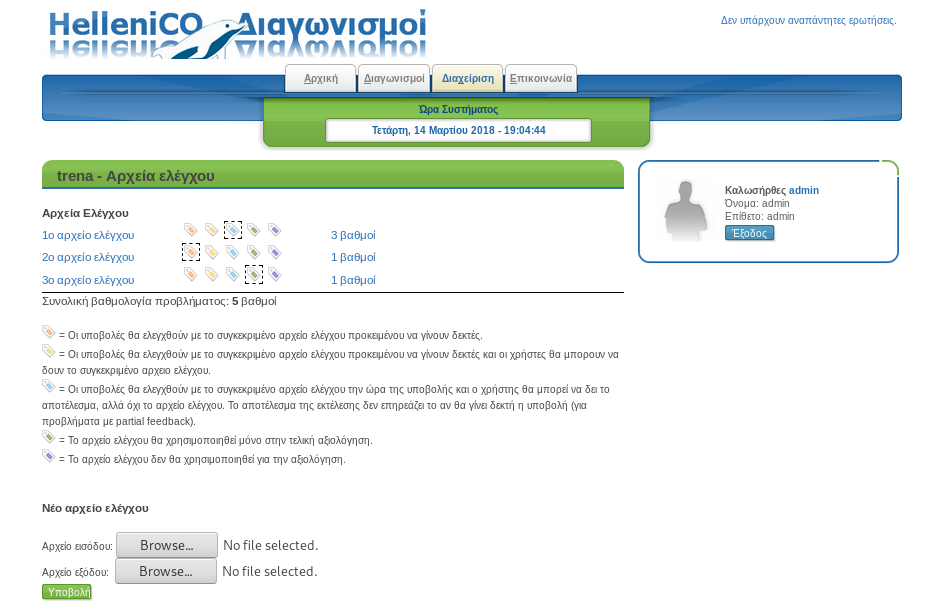
\includegraphics[scale=0.3,trim=4 4 4 4,clip]{Figures/bluetag.png}
  \caption[Οθόνη διαχείρισης προβλήματος]{Η οθόνη της διαχείρισης ενός διαγωνισμού.
  Διακρίνονται συνολικά στατιστικά για τις υποβολές, η κατάσταση της ουράς και των
  Workers.}
\end{figure}

\section{Testcase Groups}

Έχοντας προσθέσει το blue tag, τροποποιώντας πολλαπλά σημεία του Grader τόσο
για την υποβολή όσο και για την αξιολόγηση, μπορούσαμε να προχωρήσουμε στην
υλοποίηση της αρκετά πιο σύνθετης δυνατότητας, των testcase groups.

\subsection{Κίνητρο}

Πριν τις αλλαγές μας, ο διαχειριστής, κατά την δημιουργία του προβλήματος,
έπρεπε να δημιουργήσει αρχεία ελέγχου και να επιλέξει στο καθένα βαθμολογία και
τύπο εκτέλεσης. Από κείνο το σημείο και έπειτα, τα αρχεία ελέγχου δεν είχαν
κάποια κατηγοριοποίηση ή διαχωρισμό. Ο διαχειριστής, σε κάθε σημείο, όφειλε να
διατηρεί την ισορροπία όσον αφορά στις βαθμολογίες των αρχείων ελέγχου και να
θυμάται την αναλογία εύκολων και δύσκολων αρχείων ή οποιαδήποτε άλλης
κατηγορίας.

\bigskip

Άλλο ένα πρόβλημα που υπήρχε ήταν η δυνατότητα για δημιουργία ειδικών λύσεων σε
συγκεκριμένα προβλήματα έτσι ώστε να λαμβάνουν αξιοπρεπή βαθμολογία έχοντας
υλοποιήσει μέρος μόνο του αλγορίθμου, αρκεί να περνούσαν τα αναγκαία αρχεία της
κανονικής υποβολής. Κάθε αρχείο ελέγχου είχε δικιά του βαθμολογία οπότε θα
μπορούσε κανείς να επιτύχει στα μισά παραδείγματος χάρη σε ένα true/false
πρόβλημα.

\bigskip

Η προσθήκη testcase groups θα επιτρέψει την ομαδοποίηση των αρχείων ελέγχου σε
ομάδες ανεξάρτητες στην αξιολόγηση με δική τους βαθμολογία με την ορθότητα τους
να κρίνεται από την ορθότητα όλων των αρχείων ελέγχουν που περιέχουν. Έτσι, θα
δοθεί μεγάλη ευελιξία στη δημιουργία διαφορετικών κατηγοριών αρχείων. Ένας
χρήσιμος διαχωρισμός θα μπορεί να είναι ανάλογα με το μέγεθος της εισόδου,
δηλαδή σε μικρά, μεσαία και μεγάλα. Με αυτό τον τρόπο ο διαχειριστής γλιτώνει
πολύ κόπο πετυχαίνοντας την επιθυμητή αναλογία βαθμολογίας στις διάφορες
υλοποιήσεις βάζοντας απλά τους βαθμούς που θέλει ανεξάρτητα με το πόσα αρχεία
ελέγχου εμπεριέχει κάθε group.

\bigskip

Επιπροσθέτως, λύνεται το πρόβλημα των προσαρμοσμένων λύσεων, αφού αν τα
υπάρχοντα groups εμπεριέχουν αρχεία πολλαπλών περιπτώσεων, οι συγκεκριμένες
λύσεις δε θα καταφέρνουν να ικανοποιήσουν ταυτόχρονα τα αρχεία και δε θα
βαθμολογούνται σε αυτά τα groups.

\subsection{Προδιαγραφές}

Για την καθοδήγηση της υλοποίησης τέθηκαν συγκεκριμένες προδιαγραφές όσον
αφορά τις ομάδες αρχείων ελέγχου και τη λειτουργία τους.

\begin{itemize}

    \item Οι ομάδες αρχείων ελέγχου, όπως περιγράφηκαν και παραπάνω, θα μπορούν
      να περιέχουν οποιοδήποτε υποσύνολο των διαθέσιμων αρχείων. Επιθυμούμε,
      για μεγαλύτερη ευελιξία, τα αρχεία ελέγχου να μπορούν να ανήκουν σε
      πολλαπλές ομάδες και με διαφορετικό τύπο εκτέλεσης.

    \item Η αξιολόγηση θα γίνεται με βάση μόνο τις ομάδες, ανεξάρτητα με το
      πόσα αρχεία ελέγχου υπάρχουν. Μια υποβολή θα θεωρείται ορθή και θα μπορεί
      να τεθεί ως ενεργή αν ικανοποιεί τουλάχιστον μια ομάδα.

    \item Οι ομάδες θα μπορούν να αποκτήσουν τίτλο από το διαχειριστή και θα
      διαθέτουν βαθμολογία. Τα παραπάνω καθιστούν τις βαθμολογίες και τύπους
      εκτέλεσης των αρχείων ελέγχου ανούσιες.

    \item Οι ομάδες που περιέχουν τουλάχιστον ένα αρχείο ελέγχο με τύπο εκτέλεσης
      μη-τελικής αξιολόγησης, δηλαδή κίτρινο, πορτοκαλί ή μπλε, θα αξιολογούνται
      κατά τις κανονικές υποβολές και θα είναι εμφανείς στους διαγωνιζόμενους
      μαζί με τα αρχεία ελέγχου που διαθέτουν.

\end{itemize}

\subsection{Υλοποίηση}

Με βάση τις προδιαγραφές που περιγράφηκαν παραπάνω σχηματίζεται η εικόνα της
υλοποίησης και των κρίσιμων κομματιών της. Ως προς τη βάση δεδομένων, θα
χρειαστεί ένας νέος πίνακας για τα testcase groups και τα χαρακτηριστικά τους
(όνομα, βαθμολογία).

\bigskip

Δεδομένου ότι η σχέση αρχείων ελέγχου και ομάδων είναι N-to-N, δηλαδή τόσο οι
ομάδες περιέχουν πολλαπλά αρχεία και τα αρχεία ανήκουν σε πολλαπλές ομάδες, θα
χρειαστεί και δεύτερος πίνακας αντιστοίχισης ομάδων με τα αρχεία που περιέχουν.
Ο συγκεκριμένος πίνακας θα έχει και πεδίο για τον τύπο εκτέλεσης του αρχείου
ελέγχου στη συγκεκριμένη ομάδα, επιτρέποντας ένα αρχείο να ανήκει ως φανερό
(κίτρινο) σε μία ομάδα και ως τελικό (πράσινο) σε μία άλλη. Οι σχετικοί πίνακες
παρουσιάζονται στις εικόνες 38 και 39.

\bigskip

Από τη στιγμή που υπάρχει η πιθανότητα δύο ομάδες να έχουν κοινά αρχεία ελέγχου
σε πρόβλημα, δημιουργείται το θέμα της πιθανής αχρείαστης αξιολόγησης των ίδιων
αρχείων ελέγχου πολλές φορές. Στην υλοποίηση μας αυτό θα αποφευχθεί διατηρώντας
την αρχιτεκτονική της εφαρμογής όσον αφορά στις αρμοδιότητες Kewii και Grader
απαράλλαχτη. Αυτό σημαίνει ότι ο Kewii θα συνεχίσει να παίρνει απλά μια λίστα
με τα αρχεία ελέγχου που πρέπει να εκτελέσει και θα επιστρέφει το αποτέλεσμα
τους. Πρακτικά, δε θα "αντιληφθεί" την αλλαγή, καθώς ο Grader θα είναι
υπεύθυνος κατά την υποβολή μιας λύσης να φιλτράρει τα μοναδικά αρχεία ελέγχου
που του χρειάζονται για τις ομάδες που συμμετέχουν στην αξιολόγηση, και κατά το
callback για την χρησιμοποίηση αυτών των αποτελεσμάτων για να λάβει την τελική
έκβαση των testcase groups.

\bigskip

Για τη διαχείριση των testcase groups κρίθηκε αναγκαίο να δημιουργηθεί μια νέα
οθόνη για την διαχείριση και τη δημιουργία testcase groups, η οποία εισάχθηκε
στην ήδη υπάρχουσα διαχείριση αρχείων ελέγχου. Η τελευταία χρειάστηκε
σημαντικές τροποποιήσεις, καθώς πλέον τα αρχεία ελέγχου δεν μπορούν να έχουν
βαθμολογίες και τύπους εκτέλεσης (χρώματα) εκτός των ομάδων που ανήκουν. Τα
χρωματικά tags παρέμειναν, δίνοντας τη δυνατότητα στο διαχειριστή να αλλάξει
μαζικά τον τύπο ενός αρχείου ελέγχου σε όλες τις ομάδες που ανήκει. Κρίθηκε
σημαντικό η πληροφορία για τις ομάδες, τις βαθμολογίες τους και το ποια αρχεία
εμπεριέχει η κάθε μια, να εμφανίζεται στη συγκεκριμένη οθόνη χωρίς να είναι
απαραίτητη η μετάβαση στη οθόνη της διαχείρισης ομάδας αρχείων ελέγχου. Οι δύο
προαναφερθείσες οθόνες εμφανίζονται στις εικόνες 4.3 και 4.4.

\bigskip

\begin{figure}
  \centering
  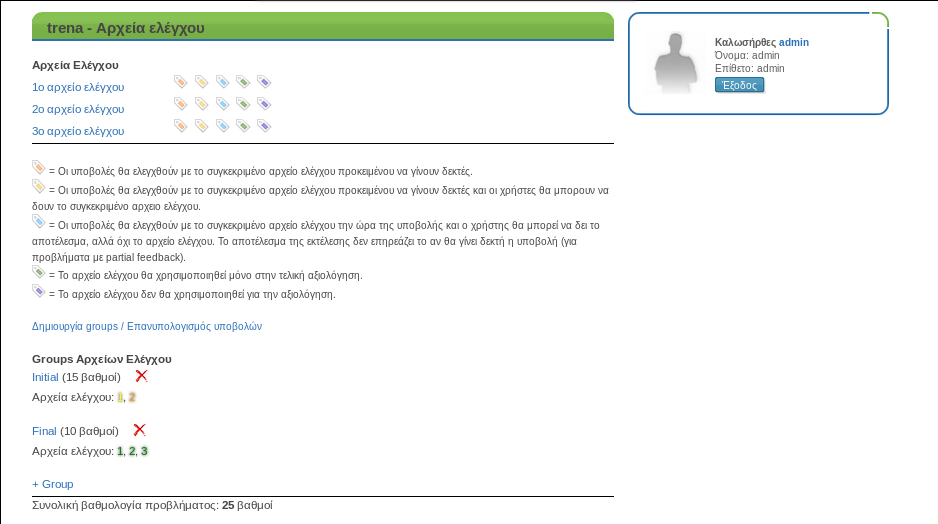
\includegraphics[scale=0.3,trim=4 4 4 4,clip]{Figures/groupoverview.png}
  \caption[Οθόνη διαχείρισης προβλήματος]{Η οθόνη της διαχείρισης ενός διαγωνισμού.
  Διακρίνονται συνολικά στατιστικά για τις υποβολές, η κατάσταση της ουράς και των
  Workers.}
\end{figure}

\begin{figure}
  \centering
  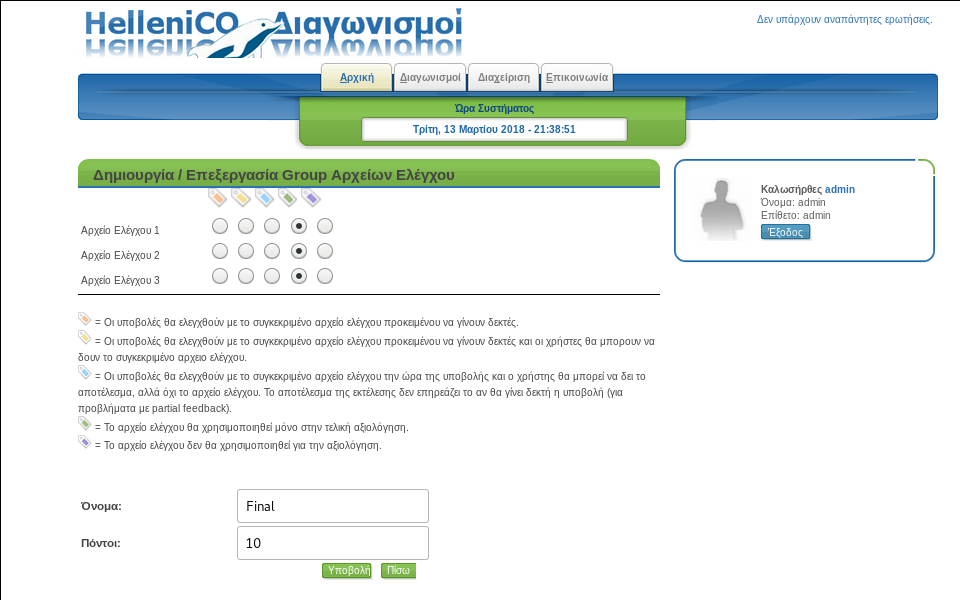
\includegraphics[scale=0.3,trim=4 4 4 4,clip]{Figures/groupedit.png}
  \caption[Οθόνη διαχείρισης προβλήματος]{Η οθόνη της διαχείρισης ενός διαγωνισμού.
  Διακρίνονται συνολικά στατιστικά για τις υποβολές, η κατάσταση της ουράς και των
  Workers.}
\end{figure}

\bigskip

Η εισαγωγή των testcase groups στο Grader επηρέασε, ακόμα, μεγάλο πλήθος οθονών
και λειτουργιών συμπεριλαμβανομένων των παρακάτω:

\begin{itemize}
    \item Αλλαγές στην οθόνη των λεπτομερειών υποβολής. Στη συγκεκριμένη
      οθόνη πλέον εμφανίζονται ομάδες αντί για αρχεία, οι οποίες περιέχουν
      τα αρχεία που αντιστοιχούν σε αυτές μέσα σε πλαίσια. Οι χρωματικές ενδείξεις
      επιτυχίας (πράσινο φόντο) και αποτυχίας (κόκκινο) έχουν παραμείνει, με την
      προσθήκη αλλαγής του φόντου του τίτλου της ομάδας ανάλογα με τη συνολική
      έκβαση.

    \item Αλλαγές στην οθόνη παρουσίασης όλων των υποβολών και επιλογής της ενεργής.
      Εδώ έπρεπε να προστεθεί μία ένδειξη ορθότητας κάθε υποβολής πέρα από τις
      υπάρχουσες, δηλαδή πράσινο/κόκκινο. Μια ορθή υποβολή θα είναι πράσινη αλλά
      μπορεί π.χ. να έχει περάσει μόνο το ένα από τα τρία testcase groups, κάτι
      που δεν είναι εμφανές μέχρι να μεταβεί ο διαγωνιζόμενος στις λεπτομέρειες
      υποβολής. Στο συγκεκριμένο παράδειγμα θα αναγράφεται 1/3.

    \item Στην οθόνη διαχείρισης προβλημάτων και διαγωνισμών άλλαξαν τα στατιστικά
      δίπλα σε κάθε πρόβλημα που έως τώρα παρουσίαζαν την αναλογία αρχείων ελέγχου
      ανά τύπο εκτέλεσης. Πλέον, εμφανίζονται μόνο δύο αριθμοί, ο συνολικός αριθμός
      αρχείων ελέγχου και ομάδων.

\end{itemize}

\begin{figure}
  \centering
  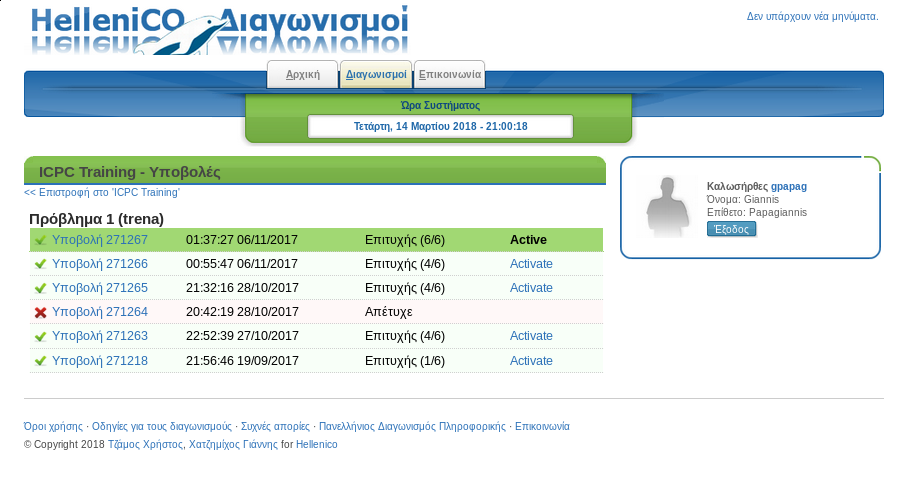
\includegraphics[scale=0.3,trim=4 4 4 4,clip]{Figures/allsubmissions.png}
  \caption[Οθόνη διαχείρισης προβλήματος]{Η οθόνη της διαχείρισης ενός διαγωνισμού.
  Διακρίνονται συνολικά στατιστικά για τις υποβολές, η κατάσταση της ουράς και των
  Workers.}
\end{figure}

\begin{figure}
  \centering
  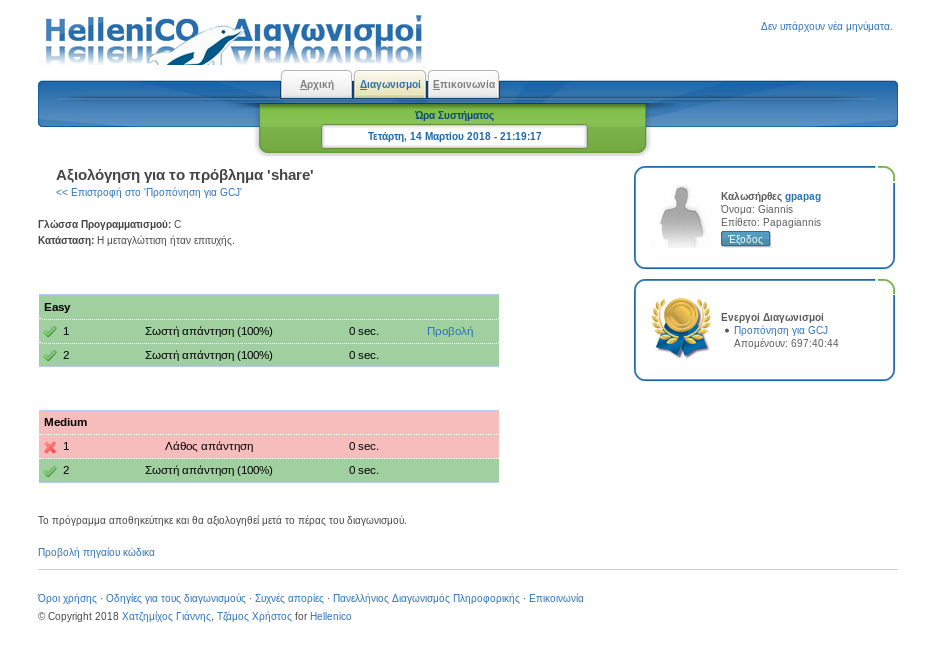
\includegraphics[scale=0.3,trim=4 4 4 4,clip]{Figures/cursubmission.png}
  \caption[Οθόνη διαχείρισης προβλήματος]{Η οθόνη της διαχείρισης ενός διαγωνισμού.
  Διακρίνονται συνολικά στατιστικά για τις υποβολές, η κατάσταση της ουράς και των
  Workers.}
\end{figure}

\bigskip

Άλλη μια σημαντική πτυχή της υλοποίησης αποτελεί ο τρόπος που θα γίνει η
μετάβαση από τον προηγούμενο τρόπο αξιολόγησης στο νέο. Εκτός από τις πολλαπλές
τροποποιήσεις στον κώδικα και στη βάση, επιβάλλεται να τροποποιηθούν όλα τα
προβλήματα, παλιά και τρέχοντα. Ο λόγος είναι ότι στο νέο σύστημα η αξιολόγηση όλων
των υποβολών βασίζεται στα testcase groups αντί για τα μεμονωμένα αρχεία ελέγχου.
Ως αποτέλεσμα, κάθε υπάρχων πρόβλημα θα πρέπει να αποκτήσει groups τα οποία,
ιδανικά, θα είναι ισοδύναμα με τα υπάρχοντα αρχεία ελέγχου.

\bigskip

Ο τρόπος να επιτευχθεί η ισοδυναμία προηγούμενης και νέας κατάστασης είναι η
δημιουργία ενός group που να περιέχει μόνο τα αρχεία ελέγχου κανονικών
υποβολών, δηλαδή μπλε, κίτρινα και πορτοκαλί, με βαθμολογία 0. Αυτή η ομάδα,
ουσιαστικά, πετυχαίνει την προσομοίωση της προηγούμενης κατάστασης όπου οι
υποβολές ελέγχονταν στα συγκεκριμένα αρχεία ελέγχου και εφόσον τα περνούσαν
όλα, η λύση ήταν σωστή και γινόταν ενεργή. Αυτή η ομάδα όμως δεν αρκεί, καθώς
χρειάζονται και ομάδες για την τελική αξιολόγηση. Αντίστοιχα, θα πρέπει να
δημιουργηθούν ακόμα ίσος αριθμός ομάδων με τα ενεργά αρχεία ελέγχου (όλα εκτός
των μωβ), και πιο συγκεκριμένα, κάθε ομάδα θα περιέχει ένα αρχείο ελέγχου με
χρώμα πράσινο και η βαθμολογία της θα είναι ίση με τη βαθμολογία του αρχείου
ελέγχου. Έτσι, πετυχαίνουμε την προσομοίωση και της τελικής αξιολόγησης, καθώς
όλες αυτές οι ομάδες δε θα ελέγχονται στην κανονική υποβολή αφού περιέχουν μόνο
πράσινα αρχεία ελέγχου (και συγκεκριμένα ένα η κάθε μία). Για τη διαδικασία
αυτή, υλοποιήθηκε script, το οποίο εισάχθηκε στην οθόνη διαχείρισης αρχείων
ελέγχου του προβλήματος.

\bigskip

Η υλοποίηση όσον αφορά στο frontend και τη λογική του Grader, συνδυάστηκε με
μερικό refactoring των κλάσεων και των συναρτήσεων, χρησιμοποιώντας πολλές από
τις αρχές που περιγράφονται στο Clean Code του Robert Martin
\cite{martin2009clean}. Μέρος των αλλαγών ήταν και η προσθήκη ενός πεδίου στον
πίνακα των υποβολών, με τίτλο resultsjson, το οποίο περιέχει τα αναλυτικά
αποτελέσματα μιας υποβολής, κωδικοποιημένα σε μορφή JSON, έτσι ώστε να μην
υπολογίζονται κάθε φορά που απαιτούνται. Επιπλέον, αλλαγές έγιναν ώστε να
αφαιρεθούν κομμάτια επαναλαμβανόμενου κώδικα με την αντίστοιχη δημιουργία νέων
δομών και κλάσεων, αποσύνδεση της λογικής διαφορετικών αντικειμένων και μείωση
της πολυπλοκότητας μεγάλων κομματιών κώδικα με δημιουργία μικρότερων
συναρτήσεων με περιγραφικά ονόματα.

\bigskip

\begin{figure}
  \centering
  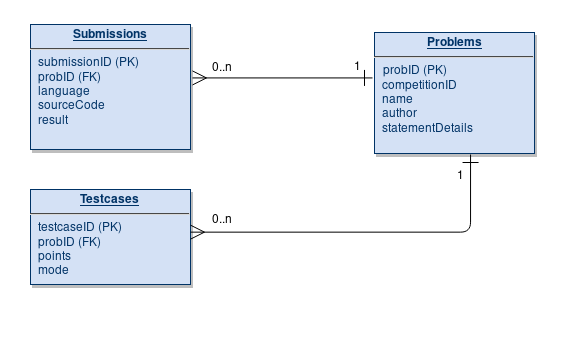
\includegraphics[scale=0.3,trim=4 4 4 4,clip]{Figures/groupsbefore.png}
  \caption[Οθόνη διαχείρισης προβλήματος]{Η οθόνη της διαχείρισης ενός διαγωνισμού.
  Διακρίνονται συνολικά στατιστικά για τις υποβολές, η κατάσταση της ουράς και των
  Workers.}
\end{figure}

\begin{figure}
  \centering
  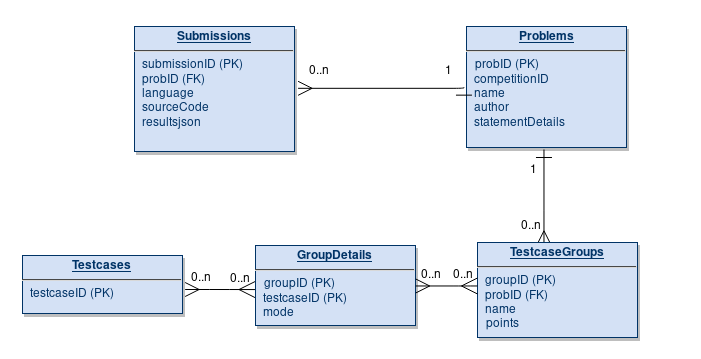
\includegraphics[scale=0.3,trim=4 4 4 4,clip]{Figures/groupsafter.png}
  \caption[Οθόνη διαχείρισης προβλήματος]{Η οθόνη της διαχείρισης ενός διαγωνισμού.
  Διακρίνονται συνολικά στατιστικά για τις υποβολές, η κατάσταση της ουράς και των
  Workers.}
\end{figure}

\chapter{Σχεδίαση για διαχωρισμό Προβλημάτων - Διαγωνισμών}

Στο παρόν κεφάλαιο θα περιγραφούν οι αλλαγές που έγιναν στο Grader για την
τροποποίηση της λογικής του με σκοπό τη βελτίωση της ευκολίας χρήσης του
στο πλαίσιο μαθημάτων προγραμματισμού και σειρών ασκήσεων. Αυτό απαιτεί την
μερική αποσύνδεση των προβλημάτων από τους διαγωνισμούς ώστε αυτά να μπορούν
να επαναχρησιμοποιηθούν. Θα αναλύσουμε πρώτα το κίνητρο για την αλλαγή αυτή
και έπειτα οι λεπτομέρειες της υλοποίησης.

\section{Κίνητρο}

Ο πρωταρχικός στόχος που δημιουργήθηκε ο Grader ήταν η χρήση του για διαγωνισμούς
πληροφορικής. Κάθε διαγωνισμός θα αποτελούσε ξεχωριστό, one-time γεγονός με
προβλήματα που θα είχαν δημιουργηθεί για αυτόν, διαγωνιζόμενους "μιας χρήσης"
και υποβολές άρρηκτα συνδεδεμένες τόσο στον διαγωνισμό όσο και στο εκάστοτε
πρόβλημα.

\bigskip

Τα προβλήματα, έπειτα από τη δημιουργία τους, παραμένουν ανένταχτα, στην κατηγορία
"Προβλήματα εκτός διαγωνισμών" της οθόνης διαχείρισης
όπως φαίνεται και στο σχήμα 5.1. Το επόμενο βήμα είναι η μετακίνηση τους
σε κάποιον διαγωνισμό με χρήση του μενού στα δεξιά του προβλήματος. Η μετακίνηση
αυτού του τύπου είναι ο μόνος τρόπος να επαναχρησιμοποιηθεί το πρόβλημα και σε
άλλους διαγωνισμούς, αφότου τελειώσει αυτός για τον οποίο δημιουργήθηκε
(ουσιαστικά, ο πρώτος στον οποίο μετακινήθηκε). Το θέμα που δημιουργείται, σε αυτό
το σημείο, είναι ότι κατά τη μετακίνηση του, το πρόβλημα διατηρεί όλες τις
προηγούμενες υποβολές του, οι οποίες πρακτικά αγνοούνται στο νέο διαγωνισμό, ενώ
ο προηγούμενος διαγωνισμός χάνει το πρόβλημα που είχε. Όλα τα παραπάνω οφείλονται
στον τρόπο που είναι σχεδιασμένη η βάση, ο οποίος παρουσιάζεται παρακάτω.

\bigskip

\begin{figure}
  \centering
  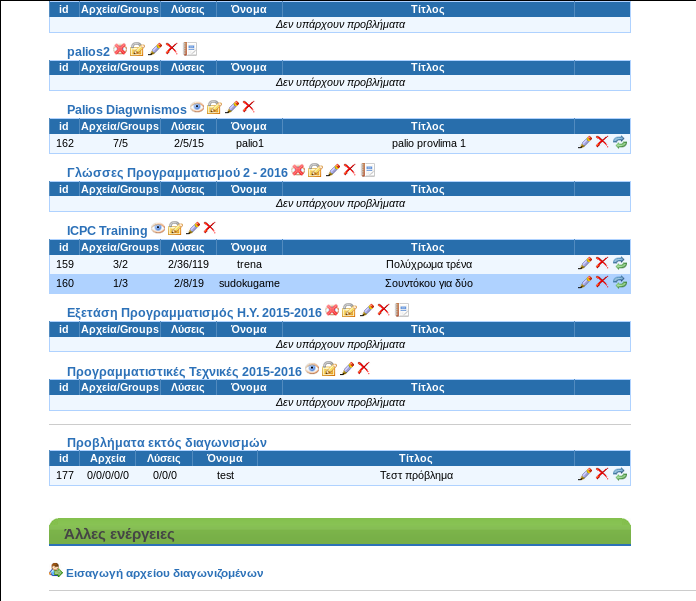
\includegraphics[scale=0.4,trim=4 4 4 4,clip]{Figures/beforesep.png}
  \caption[Η αρχιτεκτονική του CMS]{Οι υπηρεσίες του CMS και οι σχέσεις μεταξύ τους}
\end{figure}
(TODO εδώ εικόνα διαχείρισης και ισως αλλαγή αναφορών σε εικονα 1, 2 κτλ.)

\bigskip

\begin{figure}
  \centering
  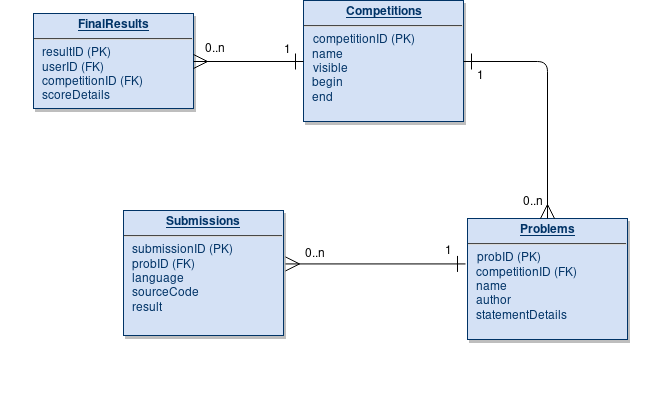
\includegraphics[scale=0.4,trim=4 4 4 4,clip]{Figures/sepbefore.png}
  \caption[Η αρχιτεκτονική του CMS]{Οι υπηρεσίες του CMS και οι σχέσεις μεταξύ τους}
\end{figure}

\bigskip

Στο σχήμα 5.2 αρχίζει να διακρίνεται το πρόβλημα που δημιουργείται. Η σύνδεση
κάθε προβλήματος με το διαγωνισμό γίνεται μέσω του πεδίο competitionID στον πίνακα
των προβλημάτων. Ως αποτέλεσμα, το μόνο που κάνει η λειτουργία της μετακίνησης
προβλήματος σε άλλον διαγωνισμό είναι να αλλάξει αυτό το πεδίο. Επιπροσθέτως,
όπως βλέπουμε, οι υποβολές συνδέονται άμεσα μόνο με τα προβλήματα και αυτός
είναι ο λόγος που μεταφέρονται μαζί με αυτά κατά τη μετακίνηση τους.

\bigskip

Τέλος, είναι αξιοσημείωτος ο τρόπος που στον πίνακα finalresults, στον
οποίο καταχωρούνται τα αποτελέσματα μετά την τελική αξιολόγηση, αποθηκεύονται
τα επιμέρους σκορ των προβλημάτων του· χωρισμένα απλά με κόμμα, σύμφωνα με μια
αύξουσα ταξινόμηση των id των προβλημάτων που περιείχε κατά την τελική αξιολόγηση.
Παραδείγματος χάρη, αν ο διαγωνισμός 15 περιέχει τα προβλήματα 48 και 51 και ένας
διαγωνιζόμενος έχει λάβει 7 βαθμούς στο πρώτο και 9 στο δεύτερο, το πεδίο score θα
έχει την τιμή 16 και το πεδίο scoreDetails θα έχει την τιμή 7,9. Όπως γίνεται
αντιληπτό, όταν αλλάξει η σύνθεση ενός διαγωνισμού, χάνεται η ιστορικότητα των
αποτελεσμάτων αφού δεν είναι δυνατό να ανακτηθεί από τη βάση η σύνδεση των
βαθμολογιών με τα προβλήματα του διαγωνισμού.

\bigskip

\section{Υλοποίηση}

Η κύρια λειτουργική αλλαγή/δυνατότητα που θα προστεθεί είναι αυτή της προσθήκης
των προβλημάτων σε νέους διαγωνισμούς χωρίς να επηρεάζονται οι προηγούμενοι.
Το κύριο μέρος της υλοποίησης για τη συγκεκριμένη δυνατότητα/βελτίωση αποτελεί
η αλλαγή στους πίνακες της βάσης και στις σχέσεις μεταξύ τους.

\bigskip

Αρχικά, θα πρέπει να δημιουργηθεί ένας πίνακας που να συνδέει κάθε διαγωνισμό
με τα προβλήματα που διαθέτει. Το πεδίο στον πίνακα των προβλημάτων που έως
τώρα χρησίμευε για αυτή τη σύνδεση, δεν αρκεί αφού πλέον θέλουμε να υπάρχει
σχέση πολλά προς ένα για προβλήματα και διαγωνισμούς. Ο νέος πίνακας χρειάζεται
απλά να περιέχει τα πεδία competitionID και probID.

\bigskip

Όπως αναφέρθηκε και παραπάνω, οι υποβολές θα πρέπει να συνδέονται με το
διαγωνισμό και όχι με το πρόβλημα. Αυτό θα επιτευχθεί με την προσθήκη του
πεδίου competitionID στον πίνακα των υποβολών. Με αυτό τον τρόπο, είναι εύκολο να
γίνει ο διαχωρισμός των υποβολών ανά διαγωνισμό και πρόβλημα ώστε κάθε πρόβλημα
να μπορεί να έχει ξεχωριστά δεδομένα υποβολών και αποτελεσμάτων σε κάθε
διαγωνισμό που ανήκει.

\bigskip

Άλλη μια αλλαγή που κρίθηκε σημαντική είναι η προσθήκη ενός πεδίου JSON στον
πίνακα των αποτελεσμάτων σε αντικατάσταση του scoreDetails. Το scoreDetailsjson
θα έχει την ίδια λογική, δηλαδή θα αναγράφει τις επιμέρους βαθμολογίες σε κάθε
πρόβλημα του διαγωνισμού. Η διαφορά θα είναι ότι δε θα σημειώνεται στη βάση μόνο
η βαθμολογία αλλά ζευγάρια probID: βαθμολογία. Στο παράδειγμα που χρησιμοποιήθηκε
προηγουμένως, το πεδίο θα έχει τη μορφή $\{48: 7, 51: 9\}$.

\bigskip

Χάρη στην προσθήκη του πεδίου scoreDetailsjson, ένας διαχειριστής θα μπορεί να δει
με λεπτομέρεια τα αποτελέσματα ενός διαγωνισμού για κάθε διαγωνιζόμενο ακόμα και
αν έχει αλλάξει η δομή του, κάτι που πριν ήταν αδύνατο. Βεβαίως, από τη στιγμή που
θα εισαχθεί η δυνατότητα αντιγραφής αντί μετακίνησης των προβλημάτων δε θα τίθεται
συχνά θέμα αλλαγής της δομής ενός διαγωνισμού μετά τον υπολογισμό αποτελεσμάτων και
την ολοκλήρωση του.

\bigskip

Έπειτα από τις αλλαγές που περιγράφηκαν, η νέα μορφή της βάσης φαίνεται στο σχήμα3.
Ο πίνακας compproblems είναι η νέα προσθήκη που είναι αναγκαία για τη σύνδεση
προβλημάτων με διαγωνισμός διατηρώντας μια κανονικοποιημένη βάση για αποφυγή του
πλεονασμού δεδομένων. (TODO: ισως αναφορα σε κατι σχετικο). Νέα πεδία προστέθηκαν,
επίσης και στους πίνακες submissions και finalresults.

\bigskip

\begin{figure}
  \centering
  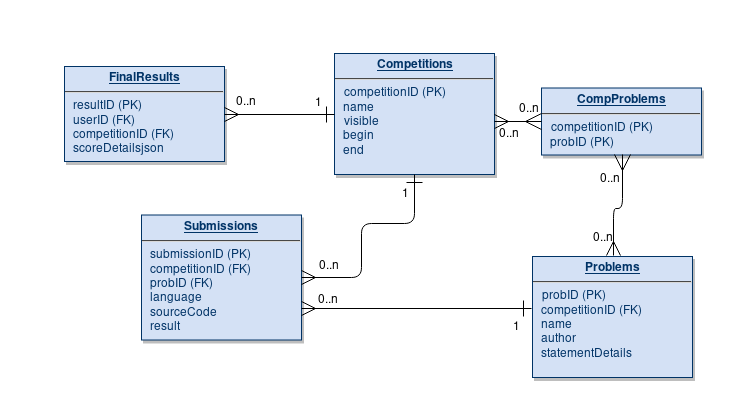
\includegraphics[scale=0.4,trim=4 4 4 4,clip]{Figures/sepafter.png}
  \caption[Η αρχιτεκτονική του CMS]{Οι υπηρεσίες του CMS και οι σχέσεις μεταξύ τους}
\end{figure}

\bigskip

(TODO: ισως subsection) Έχοντας αλλάξει τη βάση, αυτό που μένει είναι η
υλοποίηση των αλλαγών στο Grader ώστε να δίνεται η δυνατότητα της αντιγραφής
των προβλημάτων και να αξιοποιούνται τα νέα πεδία και πίνακες. Η πλειοψηφία των
αλλαγών αφορούν την οθόνη διαχείρισης, καθώς εκεί πρέπει να αλλάξει ο τρόπος
που αντιστοιχίζονται τα προβλήματα με τους διαγωνισμούς, όπως και οι υποβολές
αυτών. Ακόμα, η λειτουργία του πλήκτρου μετακίνησης αλλάζει σε αντιγραφή, πάλι
επιλέγοντας διαγωνισμό. Τέλος, στο κάτω μέρος της οθόνης, όπου αναγράφονταν τα
ανένταχτα προβλήματα, κρίθηκε προτιμότερο να αναγράφονται όλα τα προβλήματα
ώστε να είναι ευκολότερο να αναζητηθεί και να αντιγραφεί κάποιο σε ένα νέο
διαγωνισμό. Η νέα διαχείριση παρουσιάζεται στις φωτογραφίες 5.2 και 5.3.

\bigskip

\begin{figure}
  \centering
  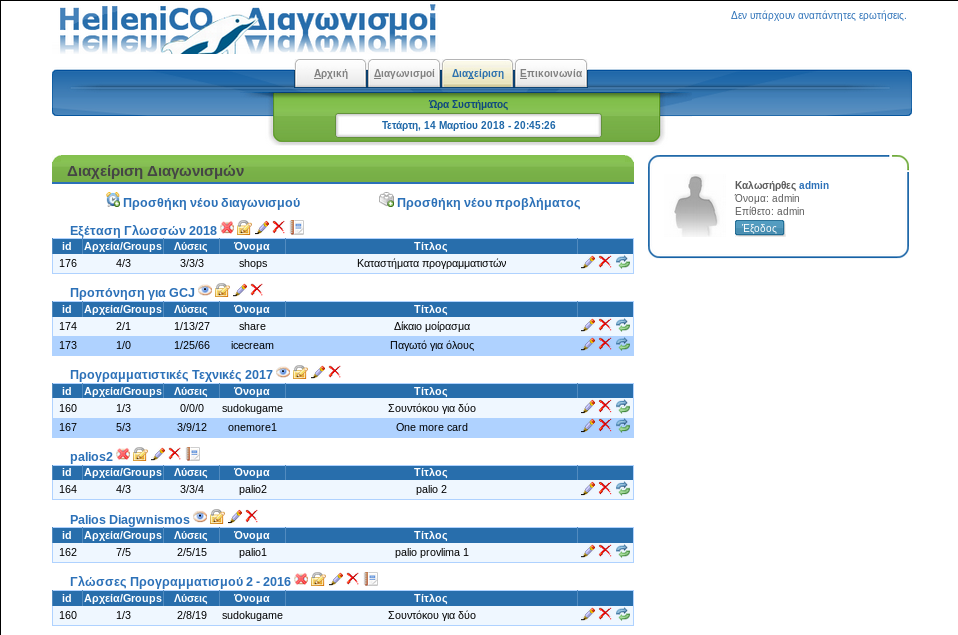
\includegraphics[scale=0.4,trim=4 4 4 4,clip]{Figures/aftersep.png}
  \caption[Η αρχιτεκτονική του CMS]{Οι υπηρεσίες του CMS και οι σχέσεις μεταξύ τους}
\end{figure}

\begin{figure}
  \centering
  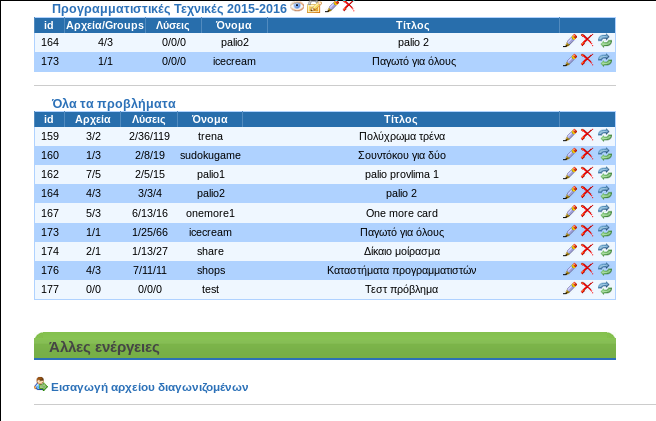
\includegraphics[scale=0.4,trim=4 4 4 4,clip]{Figures/aftersepall.png}
  \caption[Η αρχιτεκτονική του CMS]{Οι υπηρεσίες του CMS και οι σχέσεις μεταξύ τους}
\end{figure}

\bigskip

Μια ενδιαφέρουσα παρατήρηση είναι ότι η αντιγραφή ενός προβλήματος σε νέο
διαγωνισμό, απλά αλλάζει τους συσχετισμούς στη βάση, προσθέτοντας μια νέα
εγγραφή στον compproblems. Τόσο τα αρχεία ελέγχου, που είναι αποθηκευμένα στο
δίσκο του εξυπηρετητή για να διαβάζονται από τον Kewii, όσο και οι ομάδες
αρχείων ελέγχου, που αντιστοιχίζονται στη βάση με τα προβλήματα, δεν
αντιγράφονται και, ως αποτέλεσμα χαρακτηρίζουν το πρόβλημα σε όλους τους
διαγωνισμούς που αυτό ανήκει. Η σχεδιαστική επιλογή έγινε κυρίως γιατί το
πρόβλημα δεν αναμένεται να αλλάζει σημαντικά κατά την επαναχρησιμοποίηση του.
Το ενδεχόμενο να χρειαστεί κάποια αλλαγή σε πρόβλημα που ανήκει ήδη σε
παλαιότερους ή παράλληλους διαγωνισμούς δε μπορεί να αποκλειστεί, και για το
λόγο αυτό προστέθηκε ένα προειδοποιητικό μήνυμα προς όποιο διαχειριστή
επιχειρήσει τέτοιες αλλαγές.

\chapter{Λοιπές Προσθήκες}

Εκτός από τις νέες δυνατότητες που αναλύθηκαν στα προηγούμενα κεφάλαια,
υλοποιήθηκαν και αλλαγές μικρότερης πολυπλοκότητας, που δε χρειάζονται
ολόκληρο κεφάλαιο για να περιγραφούν. Οι σημαντικότερες από αυτές
θα αναφερθούν σε αυτό το κεφάλαιο.

\section{Προσθήκη γλώσσας προγραμματισμού Python}

\subsection{Προσθήκη γλωσσών στο Grader/Kewii}

% TODO: ερωτηση παπασπυρου για chroot jail

Ο Grader, όπως έχει αναφερθεί και σε προηγούμενα κεφάλαια, επιτρέπει
στους διαγωνιζόμενους την υποβολή λύσεων σε οποιαδήποτε γλώσσα
προγραμματισμού από τις υποστηριζόμενες. Οι υποστηριζόμενες γλώσσες
προγραμματισμού είναι οι παρακάτω:

\begin{itemize}
    \setlength\itemsep{0em}
    \item C
    \item C++
    \item Pascal
    \item Pazcal
    \item F\#
    \item OCaml
    \item Java
    \item Fortran
    \item Haskell
\end{itemize}

\bigskip

Η προσθήκη μιας νέας γλώσσας στο Grader δεν είναι δύσκολη διαδικασία.
Όσον αφορά στο frontend, αρκεί απλά η προσθήκη στο μενού επιλογής γλώσσας
στην υποβολή και η αντίστοιχη κωδικοποίηση (που γίνεται συνήθως με την επέκταση
των πηγαίων αρχείων της γλώσσας) που θα χρησιμοποιηθεί για την καταχώρηση της
υποβολής σε βάση και Kewii. Όπως ο Kewii δεν εμπλέκεται στη διαδικασία της
αξιολόγησης, ο Grader, αντίστοιχα, έχει καθήκον απλά να περάσει την επιλογή
της γλώσσας και τον πηγαίο κώδικα ώστε να αναλάβει ο Kewii τον έλεγχο.

\bigskip

Ο Kewii αναλαμβάνει, για κάθε υποβολή, να μεταγλωττίσει τον πηγαίο κώδικα ώστε
να παράξει το εκτελέσιμο αρχείο και έπειτα να τρέξει το εκτελέσιμο για κάθε
αρχείο ελέγχου που του έχει ζητηθεί. Η μεταγλώττιση και η εκτέλεση των υποβολών
γίνεται σε ένα περιορισμένο περιβάλλον, με τη χρήση μόνο των αναγκαίων
μεταγλωττιστών και βιβλιοθηκών. Για την προσθήκη μιας γλώσσας θα πρέπει να
εγκατασταθούν στο συγκεκριμένο περιβάλλον τα αντίστοιχα εκτελέσιμα και να
τροποποιηθεί ένα αρχείο διαμόρφωσης που περιέχει τις αντιστοιχίσεις γλωσσών
και εντολών μεταγλώττισης/εκτέλεσης.

\subsection{Επιλογή Python}
% TODO: ερωτηση παπασπυρου για φακτορ παηθον

Η Python είναι μια interpreted προγραμματιστική γλώσσα υψηλού επιπέδου
γενικού σκοπού. Διαθέτει πολύ πλούσια βιβλιοθήκη για μια ευρεία γκάμα
λειτουργιών και επιστημονικών πεδίων. Έχει σχεδιαστεί με έμφαση στην
αναγνωσιμότητα και στη χρησιμοποίηση λιγότερου κώδικα, ενώ ευνοεί πολλαπλά
προγραμματιστικά στυλ όπως είναι ο δομημένος, ο αντικειμενοστρεφής και ο συναρτησιακό προγραμματισμός.

\bigskip

Δεδομένης της δημοτικότητας της Python και της ευκολίας χρήσης της, είναι μια
απαραίτητη προσθήκη στο Grader που πιθανότατα θα εκτιμηθεί από διαγωνιζόμενους
μαθητές και φοιτητές. Η Python δε λείπει από κανένα από τα συστήματα
αξιολόγησης που μελετήθηκαν, ενώ πλέον αποτελεί τη δημοφιλέστερη επιλογή στα
κορυφαία αμερικάνικα πανεπιστήμια όσον αφορά στα εισαγωγικά μαθήματα των
τμημάτων επιστήμης των υπολογιστών \cite{website:popularpython}.  Είναι μια από
τις πιο αναπτυσσόμενες προγραμματιστικές γλώσσες σύμφωνα με στοιχεία του Stack
Overflow \cite{website:pythongrowth} χάρη, κυρίως, στην καθιέρωση της σε πολλά
προγράμματα προπτυχιακών σπουδών και στην ανάπτυξη των τομέων της ανάλυσης
δεδομένων και μηχανικής μάθησης, στους οποίους κυριαρχεί ως εργαλείο
\cite{website:whypython}.

\bigskip

Η διαφορά της Python με τις γλώσσες που υποστηρίζει ο Kewii είναι ότι αυτή
αποτελεί μια interpreted γλώσσα και ως αποτέλεσμα δεν έχει ιδιαίτερο νόημα η
μεταγλώττιση της σε ένα εκτελέσιμο. Σε κάθε υποβολή με χρήση της, θα γίνεται
απευθείας εκτέλεση με είσοδο τα αρχεία ελέγχου και θα εμφανίζονται μόνο τα
σφάλματα κατά τον χρόνο εκτέλεσης στον διαγωνιζόμενο, αντίθετα με τις υπόλοιπες
γλώσσες που υπάρχουν και σφάλματα μεταγλώττισης. Στο μέλλον θα μπορούσε να
διερευνηθεί η δυνατότητα ενός εργαλείου ανάλυσης του πηγαίου κώδικα για τη
διευκόλυνση των διαγωνιζόμενων με καλύτερα μηνύματα σφαλμάτων.

\bigskip

Η έκδοση της Python που επιλέχθηκε είναι η 2.7. Η υποστήριξη της συγκεκριμένης
έκδοσης και γενικά της Python 2 θα διαρκέσει έως το 2020, οπότε καλό θα είναι
να προστεθεί και η Python 3 στο μέλλον. Δεδομένης της δουλειάς που έγινε για
την προσθήκη της έκδοσης 2, η προσθήκη της 3 θα είναι αρκετά εύκολη και άμεση.

\section{Μαζικό ανέβασμα αρχείων ελέγχων/ομάδων}

\subsection{Κίνητρο}

Κατά τη διαδικασία δημιουργίας ενός προβλήματος, είναι απαραίτητο να προστεθεί
ένας συχνά μεγάλος αριθμός αρχείων ελέγχου. Ο μόνος τρόπος να γίνει αυτό είναι
μέσω της οθόνης διαχείρισης των αρχείων ελέγχου, όπως φαίνεται στη
φωτογραφία 4.1, και κάθε νέο αρχείο ανεβαίνει ξεχωριστά, δηλαδή δεν υπάρχει
κάποια μαζική διαδικασία.

\bigskip

Για να αποφευχθεί η επαναληπτική και χρονοβόρα διαδικασία, οι έως τώρα διαχειριστές
έγραφαν απλά PHP scripts για την ενημέρωση της βάσης με τα νέα αρχεία ελέγχου,
και αντέγραφαν τα τελευταία, χειροκίνητα, στους αντίστοιχους φακέλους του Kewii.
Μετά την προσθήκη των ομάδων αρχείων ελέγχου, στη διαδικασία αυτή προστέθηκε και
η δημιουργία και παραμετροποίηση των ομάδων με τα επιθυμητά αρχεία και tags.

\bigskip

Για τους παραπάνω λόγους κρίθηκε αναγκαία η προσθήκη ενός αυτοματοποιημένου
τρόπου μαζικής προσθήκης αρχείων για τα προβλήματα, στο οποίο να υπάρχει και η
δυνατότητα ορισμού των κατάλληλων ομάδων αρχείων ελέγχου. Το εργαλείο που θα
υλοποιηθεί θα οφείλει τόσο να ενημερώνει τη βάση, όσο και να φορτώνει τα αρχεία
στον εξυπηρετητή του Kewii. Για την επεξεργασία των ομάδων, θα πρέπει να
χρησιμοποιηθεί ένα περιγραφικό αρχείο, ιδανικά σε ένα ανθρωπίνως αναγνώσιμο
τύπο αρχείου με σκοπό την εύκολη δημιουργία του.

\subsection{Υλοποίηση}

Το εργαλείο που περιγράφηκε θα προστεθεί στην οθόνη διαχείρισης των αρχείων
ελέγχου κάτω από το ήδη υπάρχον ανέβασμα μεμονωμένου αρχείου. Μετά την προσθήκη
η οθόνη θα έχει τη μορφή της φωτογραφίας 6.1. Ο διαχειριστής θα ανεβάζει ένα
συμπιεσμένο αρχείο (zip) με τα αρχεία εισόδου και εξόδου που θέλει να προσθέσει
στο πρόγραμμα. Στο αρχείο θα πρέπει, επιπλέον, να υπάρχει και ένα αρχείο με
όνομα descriptor.json το οποίο θα αναλαμβάνει να περιγράψει στο εργαλείο τις
προδιαγραφές αρχείων και ομάδων.

\bigskip

Η μορφή JSON επιλέχθηκε για τους λόγους που αναφέρθηκαν παραπάνω, δηλαδή για τα
χαρακτηριστικά της, ως αναγνώσιμη και με δυνατότητα εύκολης εισαγωγής αντικειμένων
και λιστών. Στο συγκεκριμένο αρχείο θέλαμε να περιγράφονται τα παρακάτω:

\begin{itemize}
    \item Ο τρόπος ονομασίας των αρχείων ελέγχου για τα αρχεία εισόδου και εξόδου

    \item Το πλήθος των ομάδων αρχείων ελέγχου

    \item Για κάθε ομάδα αρχείων ελέγχου το όνομα της, οι πόντοι
      και τα αρχεία ελέγχου που περιέχει

    \item Για κάθε αρχείο ελέγχου μέσα σε ομάδα ο τύπος εκτέλεσης του (tag)

\end{itemize}

Ο Grader περιμένει να βρει μέσα στο συμπιεσμένο αρχείο ζευγάρια εισόδου-εξόδου
για κάθε αρχείο ελέγχου που πρέπει να προστεθεί. Επομένως, θα πρέπει να είναι
γνωστή η μορφή των ονομάτων των αρχείων. Για μεγαλύτερη ευελιξία,
δημιουργήθηκαν δύο προαιρετικά πεδία, για αρχεία εισόδου και εξόδου αντίστοιχα,
τα οποία δέχονται τη μορφή ονομασίας που θα χρησιμοποιηθεί με χρήση ενός format
παρόμοιου με το printf της PHP. Προφανώς, αυτό θα πρέπει να περιέχει ένα
προσδιοριστή για ακέραιους αριθμούς ώστε να λειτουργεί σωστά η αντικατάσταση
για την παραγωγή των ονομασιών των αρχείων. Αν τα πεδία αυτά δεν έχουν
συμπληρωθεί χρησιμοποιείται η προεπιλεγμένη μορφή, δηλαδή probname.in1 και
probname.out2, για το πρώτο αρχείο εισόδου και εξόδου ενός προβλήματος με όνομα
probname.

\bigskip

Όσον αφορά στις ομάδες αρχείων ελέγχου, αυτές πρέπει να περιέχονται μέσα στο
descriptor.json σαν λίστες αντικειμένων. Κάθε αντικείμενο που αντιστοιχεί σε
μια νέα ομάδα, έχει πεδία για το όνομα της, τους πόντους που αξίζει και τα
αρχεία ελέγχου που θα περιέχει. Το τελευταίο πεδίο αποτελεί λίστα και περιέχει
αντικείμενα με δύο πεδία: αριθμός αρχείου ελέγχου και τύπος εκτέλεσης. Ο τύπος
εκτέλεσης θα δίνεται με το όνομα του χρώματος δηλαδή θα μπορεί να έχει τις
τιμές orange, yellow, blue, green, purple. Ακολουθεί ένα πρότυπο
descriptor.json στο οποίο έχουν συμπληρωθεί όλα τα διαθέσιμα πεδία.

\lstinputlisting[caption=Παράδειγμα descriptor.json]{Listings/descriptordiploma.json}

\begin{figure}
  \centering
  
\includegraphics[scale=0.4,trim=4 4 4 4,clip]{Figures/massupload.png}
  \caption[Η αρχιτεκτονική του CMS]{Οι υπηρεσίες του CMS και οι σχέσεις μεταξύ τους}
\end{figure}

\subsection{Εργαλείο δημιουργίας}

Χάρη στην αναγνώσιμη μορφή του JSON είναι εύκολο ένας διαχειριστής να συντάξει
ένα JSON αρχείο για το ανέβασμα αρχείων ελέγχου και καθορισμό ομάδων. Παρόλα
αυτά, θα είναι αρκετά χρήσιμο το συγκεκριμένο αρχείο να μη συντάσσεται με το
χέρι, ώστε να μην υπάρχει και η πιθανότητα σφάλματος. Για το λόγο αυτό
δημιουργήθηκε ένα interactive script σε Python για την αυτόματη παραγωγή ενός
descriptor.json αρχείου.

\bigskip

Το συγκεκριμένο script, μόλις εκτελεστεί, σε οποιοδήποτε περιβάλλον, διατυπώνει
ερωτήσεις σχετικές με τον αριθμό και τα ονόματα των αρχείων ελέγχου και ομάδων
και έπειτα για κάθε ομάδα σχετικά με το ποια αρχεία περιέχει και τους τύπους
εκτέλεσης τους. Στο τέλος, παράγει το αρχείο που περιγράφηκε. Παρακάτω φαίνεται
μια τυπική εκτέλεση του συγκεκριμένου script.


\begin{figure}
  \centering
  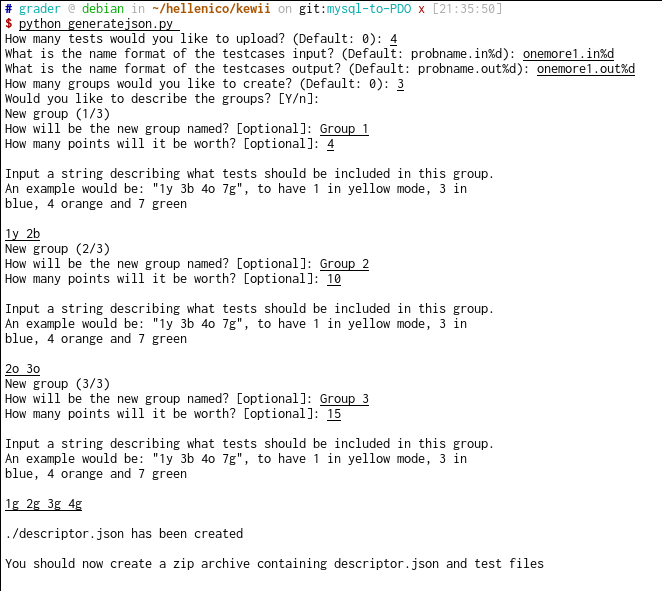
\includegraphics[scale=0.4,trim=4 4 4 4,clip]{Figures/interactive.png}
  \caption[Παράδειγμα χρήσης interactive generator script]{Οι υπηρεσίες του CMS και οι σχέσεις μεταξύ τους}
\end{figure}

\section{Αλλαγή MySQL connector}

Μια τροποποίηση που θεωρήθηκε απαραίτητη ήταν η αλλαγή της επέκτασης
επικοινωνίας της PHP με τη MySQL βάση δεδομένων μας. Η επέκταση, που
χρησιμοποιείται τόσο από τον Grader όσο και από τον Kewii, είναι το πρωτότυπο
(original) MySQL API. Το συγκεκριμένο API έχει αρκετά μειονεκτήματα, που έχουν
οδηγήσει και στην παύση της υποστήριξης του όπως περιγράφεται στο (TODO:
https://wiki.php.net/rfc/mysql\_deprecation).

\bigskip

Δεδομένου ότι η συγκεκριμένη επέκταση δεν συντηρείται πλέον και ακόμα χειρότερα
εμφανίζει E\_DEPRECATED σφάλματα ήδη από την έκδοση 5.5 της PHP (στην 7 δεν
υπάρχει), είναι επιτακτικό να αφαιρεθεί από τον κώδικα της εφαρμογής μας και να
αντικατασταθεί με μια πιο σύγχρονη. Οι επίσημα υποστηριζόμενες επεκτάσεις που
μπορούμε να χρησιμοποιήσουμε είναι οι mysqli και PDO
(https://secure.php.net/manual/en/mysql.php). Για την επιλογή χρησιμοποιήθηκε ο
παρακάτω πίνακας σύγκρισης των προαναφερθέντων επεκτάσεων που υπάρχει στο
manual της PHP (https://secure.php.net/manual/en/mysql.php TODO).

\begin{figure}
  \centering
  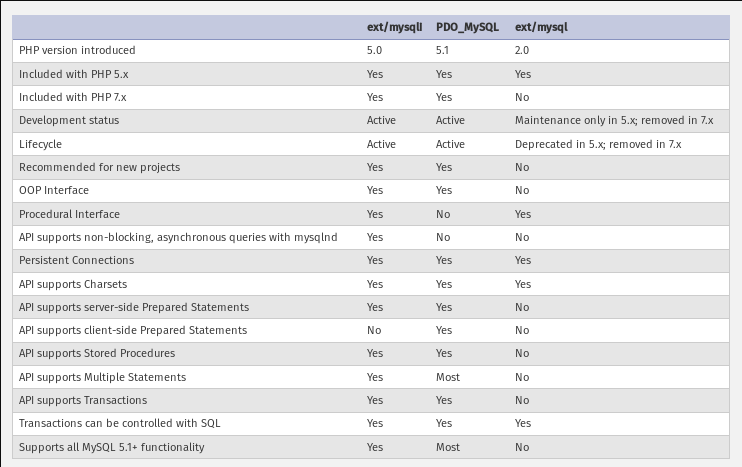
\includegraphics[scale=0.4,trim=4 4 4 4,clip]{Figures/mysqlconnectors.png}
  \caption[Παράδειγμα χρήσης interactive generator script]{Οι υπηρεσίες του CMS και οι σχέσεις μεταξύ τους}
\end{figure}

\bigskip

Όπως βλέπουμε, τόσο το mysqli όσο και το PDO υποστηρίζονται και προτείνονται
για νέες υλοποιήσεις. Κάτι που δεν γίνεται εμφανές στο συγκεκριμένο πίνακα
είναι το γεγονός ότι το PDO αποτελεί μια γενικευμένη διεπαφή ή οποία διαθέτει
οδηγούς για πολλές διαφορετικές βάσεις δεδομένων εκτός από την SQL,
προσφέροντας στο χρήστη ένα API υψηλού επιπέδου και επιτρέποντας του να αλλάξει
πολύ εύκολα βάση δεδομένων, αν χρειαστεί. Και οι δύο επεκτάσεις έχουν αρκετές
δυνατότητες που μας ενδιαφέρει να υλοποιηθούν με σημαντικότερη αυτή των
prepared statements.

\bigskip

Τα prepared statements επιτρέπουν την εκτέλεση συγκεκριμένων επερωτημάτων
(queries) με αντικατάσταση των παραμέτρων που αλλάζουν κάθε φορά. Αυτό έχει δύο
σημαντικά πλεονεκτήματα. (http://php.net/manual/en/pdo.prepared-statements.php
TODO) Αρχικά, αυξάνει ιδιαίτερα την απόδοση στην εκτέλεση διαδοχικών queries
βασισμένων στο ίδιο prepared statement. Επιπλέον, αυξάνει πολύ την ασφάλεια της
εφαρμογής μας, καθώς αποκλείει ουσιαστικά την πιθανότητα επίθεσης έκχυσης
(injection) κώδικα SQL.

\bigskip

Η επίθεση με SQL injection γίνεται δυνατή λόγω του τρόπου που δημιουργείται το
κάθε query. Αν δεν ελεγχθεί σωστά η είσοδος του χρήστη, υπάρχει η περίπτωση ο
τελευταίος να εκμεταλλευτεί ειδικούς χαρακτήρες της SQL, π.χ. τον χαρακτήρα που
ξεκινάει ένα σχόλιο, και να αλλοιώσει το Query, επηρεάζοντας την εκτέλεση και
επιτυγχάνοντας, ιδανικά, την πρόσβαση σε ευαίσθητα δεδομένα ή σελίδες.

\bigskip

Ο τρόπος που επιτυγχάνεται η αντοχή στις προαναφερθείσες επιθέσεις βασίζεται
τρόπος λειτουργίας των prepared statements. Σε πρώτη φάση, δημιουργείται το
πρότυπο επερώτημα δίχως τις παραμέτρους και μεταγλωττίζεται ξεχωριστά. Οι
παράμετροι, στέλνονται ξεχωριστά με διαφορετικό πρότυπο επικοινωνίας με
αποτέλεσμα να μην είναι δυνατόν να εισαχθούν ειδικοί χαρακτήρες που θα
επηρεάσουν την εκτέλεση του query.

\bigskip

Για την υλοποίηση επιλέχθηκε, τελικά, το PDO για τους λόγους επεκτασιμότητας
που αναφέρθηκαν παραπάνω δεδομένου ότι στα υπόλοιπα κριτήρια δεν υστερεί σε
σχέση με το mysqli, και η υπάρχουσα σχεδίαση μας είναι αντικειμενοστρεφής ούτως
ή άλλως, που υποστηρίζεται από το PDO (που δεν υποστηρίζει δομημένο στυλ).

\subsection{Συνοπτική περιγραφή επέκτασης PDO}

Η επέκταση PDO (PHP Data Objects), αποτελεί μια μικρού μεγέθους, συνεπή (για
τις διαφορετικές βάσεις δεδομένων) διεπαφή για την πρόσβαση και χρήση βάσεων
δεδομένων σε PHP. Μέσω των διάφορων, χαμηλού επιπέδου, οδηγών της επιτρέπει την
ενοποίηση του πλήθους των μεθόδων κάθε βάσης σε μια κοινή, πλούσια διεπαφή που
περιστρέφεται γύρω από κοινά αντικείμενα που αντιστοιχούν σε κάθε πίνακα ξεχωριστά.
(http://php.net/manual/en/intro.pdo.php).

\bigskip

Η σχεδίαση της συγκεκριμένης επέκτασης έχει γίνει με έμφαση στην ευκολία χρήσης
και την επαναχρησιμοποίηση του ίδιου κώδικα για διαφορετικές βάσεις δεδομένων
και συναφείς λειτουργίες. Η σύνδεση στην εκάστοτε βάση δεδομένων γίνεται με τη
χρήση μιας σειριακής δομής δεδομένων, με όνομα Data Source Name
(https://en.wikipedia.org/wiki/Data\_source\_name), έπειτα από την οποία,
δημιουργείται ένα αντικείμενο που αντιστοιχεί στη σύνδεση. Τα queries
εκτελούνται με τη χρήση της μεθόδου query, εκτός αν χρησιμοποιηθούν prepared
statements (PDOStatement), όπου χρησιμοποιούνται οι μέθοδοι prepare και
execute. Η επέκταση εμπεριέχει, επίσης, και δική της κλάση εξαιρέσεων
(PDOException). (https://secure.php.net/manual/en/book.pdo.php) Ακολουθούν
παραδείγματα απλών λειτουργιών χρησιμοποιώντας τη συγκεκριμένη επέκταση/API.


\lstinputlisting[caption=Παραδείγματα χρήσης PDO]{Listings/pdoexamples.php}

\chapter{Συμπεράσματα}

\section{Καταληκτικές Παρατηρήσεις}

Στη συγκεκριμένη εργασία έγινε μια προσπάθεια βελτίωσης του συστήματος
αυτόματος αξιολόγησης Grader και προσθήκης δυνατοτήτων που θα το καταστήσουν
πιο ευέλικτο και εύκολο στη χρήση του. Για να επιτευχθεί αυτό, διερευνήθηκε ο
τρόπος λειτουργίας του όπως και ο τρόπος λειτουργίας άλλων παρόμοιων
συστημάτων. Για τις τροποποιήσεις και τις προσθήκες που υλοποιήθηκαν, έγινε
προσπάθεια να χρησιμοποιηθούν σωστές σχεδιαστικές επιλογές με έμφαση στη
βελτίωση της ποιότητας του κώδικα, στην μετέπειτα ευκολία συντήρησης και
επέκτασης του.

\bigskip

Στο Κεφάλαιο 2, παρουσιάστηκαν συστήματα αυτόματης αξιολόγησης ανοιχτού λογισμικού
που προσφέρονται για τη διενέργεια διαγωνισμών και λειτουργούν με παρόμοιο τρόπο
με το Grader. Αναλύθηκε η σχεδίαση τους, τα σενάρια χρήσης τους και οι διαφορές
τους με το δικό μας σύστημα.

\bigskip

Στο κεφάλαιο 3, είδαμε τον τρόπο λειτουργίας του Grader και του Kewii, της
εφαρμογής που τρέχει στον εξυπηρετητή και αναλαμβάνει την εκτέλεση των
υποβληθέντων προγραμμάτων. Αναλύθηκε η αρχιτεκτονική και ο τρόπος επικοινωνίας
μεταξύ τους. Αναφέρθηκαν, ακόμα, όλα τα συστατικά στοιχεία του συστήματος, οι
σχέσεις τους και κατά πόσο εμπλέκονται με Kewii και Grader. Το συγκεκριμένο
κεφάλαιο έχει σκοπό να λειτουργήσει στο μέλλον σαν έγγραφο αναφοράς για όποιον
επιθυμεί να επεκτείνει το σύστημα, βοηθώντας τον να αντιληφθεί γρηγορότερα τον
σχεδιασμό του.

\bigskip

Στα κεφάλαια 4,5 και 6, αναλύθηκαν οι σημαντικότερες αλλαγές που έγιναν κατά τη
διάρκεια της παρούσας εργασίας. Αυτές συμπεριλάμβαναν τη δημιουργία μιας νέας
έννοιας για το σύστημα, αυτής των ομάδων αρχείων ελέγχου, και ως αποτέλεσμα την
επέκταση ολόκληρου του συστήματος για την υποστήριξη του, την αλλαγή της
αρχιτεκτονικής προβλημάτων, διαγωνισμών και υποβολών προς διευκόλυνση της
λειτουργίας του Grader και ένα σύνολο άλλων, μικρότερης σημασίας, προσθηκών.
Κατά τη διαδικασία υλοποίησης κάθε τροποποίησης έγινε προσπάθεια βελτίωσης της
εκάστοτε διαμόρφωσης με αναδιαμόρφωση κλάσεων μεθόδων και δομών δεδομένων ώστε
ο κώδικας να είναι περισσότερο κατανοητός και διαχειρίσιμος από τους μελλοντικούς
συντηρητές του. Επίσης, καταγράφηκε η διαδικασία εγκατάστασης της συνολικής
εφαρμογής του σε ένα καινούριο σύστημα ώστε να είναι εύκολο να μετεγκατασταθεί
στο μέλλον ή να δημιουργηθεί περιβάλλον δοκιμών. (TODO: πρώτη φορά τα αναφέρω αυτά!)

\section{Μελλοντική Εργασία}

Υπάρχουν πολλές προσθήκες που θα μπορούσαν να γίνουν σε Grader και Kewii για τη
βελτιστοποίηση τους. Όσον αφορά στον πρώτο, θα μπορούσε να προστεθεί η δυνατότητα
επισκόπησης και σχολιασμού υποβληθέντων λύσεων (code reviews) όπου οι διαχειριστές
ή υπεύθυνοι για τους διαγωνισμούς θα μπορούσαν να σχολιάζουν τις λύσεις των
διαγωνιζόμενων και εκεί να γίνεται συζήτηση μεταξύ τους για τυχόν βελτιστοποιήσεις
ή σφάλματα.

\bigskip

Επιπροσθέτως, θα ήταν αρκετά θετικό αν μπορούσε να διενεργηθεί ένας επανασχεδιασμός
της διαδικτυακής εφαρμογής σύμφωνα με μια αρχιτεκτονική MVC ή παρόμοια με χρήση
κάποιου σύγχρονου πλαισίου (framework) ώστε να γίνει άμεσα πιο κατανοητός ο
διαχωρισμός παρουσίασης και υλοποίησης της λογικής της αξιολόγησης και των
υπόλοιπων λειτουργιών. Κάτι τέτοιο θα είχε ως προϋπόθεση πλήρη κατανόηση του Grader
και του συνόλου των μερών του, αλλά θα επιβράβευε άμεσα όσους θα ήταν υπεύθυνοι για
την περαιτέρω ανάπτυξη του.

\bigskip

Μελλοντικά, θα μπορούσε να υπάρξει βελτίωση και του Kewii σε αρκετά θέματα.
Αρχικά, όπως έχει αναφερθεί και στο κεφάλαιο 6.1.2 για την Python, οι
διαγωνιζόμενοι θα επωφελούνταν στην περίπτωση προσθήκης ενός μηχανισμού για
ανάλυση του πηγαίου κώδικα των υποβολών τους, καθώς δεν εκτελείται μεταγλώττιση
και όλα τα σφάλματα είναι κατά την εκτέλεση. Ένα εργαλείο που θα μπορούσε να
χρησιμοποιηθεί για το συγκεκριμένο σκοπό είναι το pylint (TODO:
https://www.pylint.org/). Το συγκεκριμένο πρόγραμμα, έχει τη δυνατότητα τόσο να
εντοπίζει σφάλματα πριν την εκτέλεση, όσο και να ελέγχει την ποιότητα του
κώδικα σύμφωνα με συγκεκριμένα στάνταρ όπως είναι π.χ. το PEP-8 (TODO: link).

\bigskip

Άλλο ένα θέμα που επιδέχεται βελτίωση είναι η ασφάλεια εκτέλεσης του Kewii.
Προφανώς, είναι αρκετά δύσκολο να επιτυγχάνεται η απόλυτη ασφάλεια όταν εξ ορισμού
εκτελείται άγνωστος κώδικας σε έναν εξυπηρετητή. Παρόλα αυτά, μπορεί να υλοποιηθεί
ένα πιο αποκλεισμένο (sandboxed) περιβάλλον, πιθανόν με τη χρήση ενός εικονικού
μηχανήματος που να έχει ως στόχο τον αποκλεισμό των εκτελούμενων προγραμμάτων ή
με χρήση ειδικευμένου λογισμικού ως container, π.χ. Docker (TODO: link).

\bigskip

Τέλος, θα ήταν ωφέλιμο για την απόδοση του Kewii να υλοποιηθεί μια παραλληλοποίηση
των εκτελέσεων πολλαπλών υποβολών ταυτόχρονα, που θα μείωνε σε μεγάλο βαθμό το
χρόνο εκτέλεσης, εάν χρησιμοποιούνταν με χρήση συστάδας εικονικών ή φυσικών
μηχανημάτων. Η συγκεκριμένη υλοποίηση έχει ήδη γίνει στο (TODO: τσιαμητρος) και
είναι συμβατή με το σύστημα μας. Μένει να διερευνηθούν οι λεπτομέρειες της
προσθήκης και να διεξαχθεί αξιολόγηση της λειτουργίας.
%%%  Bibliography

\bibliographystyle{softlab-thesis}
\bibliography{thesis}

%%%  End of document

\end{document}
